


% 
% \input{sections/motivacao}
% \input{sections/problema}
% \input{sections/objetivos}
% \input{sections/contribuicoes}
% \input{sections/producao}
% %\input{sections/organizacao}
% \input{sections/conclusao}
% \input{sections/referencias}

\part{Conteúdo~da~prova~I}
\frame{\partpage}

\section{Introdução e motivação}

\begin{frame}{}
    \fontsize{14pt}{15.2}\selectfont{
	Apresentação pessoal, integração com a turma, introdução de conceitos básicos de programação de computadores e despertar curiosidade dos alunos sobre o tema.
	
	\vspace{1em}
	}\par
	\vspace{1em}
\end{frame}


\begin{frame}{Aplicação de Avaliação}
    \fontsize{14pt}{15.2}\selectfont{
	Datas importantes
	\vspace{1em}
	}\par
	
	\fontsize{12pt}{15}\selectfont{
	\begin{itemize}%[<+->]  
	    \item xx/xx/2019 - Simulado da Primeira Avaliação (1A)
	    \item \textbf{xx/xx/2019 - Primeira Avaliação}
	    \item xx/xx/2019 - Apresentação dos resultados da 1A
	    \item xx/xx/2019 - Simulado da Segunda Avaliação (2A)
	    \item \textbf{xx/xx/2019 - Segunda Avaliação}
	    \item xx/xx/2019 - Apresentação geral dos resultados
	    \item \textbf{xx/xx/2019 - Segunda Chamada}
	\end{itemize}
	
	}\par
	
	\vspace{1em}
\end{frame}



\begin{frame}{Compromisso semanal}
%     \fontsize{14pt}{15.2}\selectfont{
% 	Datas importantes
% 	\vspace{1em}
% 	}\par
	
	\fontsize{12pt}{15}\selectfont{
	\begin{itemize}%[<+->]  
	    \item Encontros: quintas e sextas
	    \item Período: 08/08/2019 à 20/12/2019
	    \item Início: 19h
	    \item Térmico: 21h30m
	    \item Intervalo: 20h10m até 20h20m (a discutir)
	    \item Sala: 28
	    \item Cada dia são três aulas: 
	        \begin{itemize}%[<+->]  
        	    \item 19h-19h50m
        	    \item 19h50m-20h40m
        	    \item 20h40m-21h30m
        	\end{itemize}
	\end{itemize}
	
	}\par
	
	\vspace{1em}
\end{frame}


\begin{frame}{Metodologia das Aulas}

	\fontsize{11pt}{15}\selectfont{
	\begin{itemize}%[<+->]  
	    \item Resolução de dúvidas gerais: 19h até 19h20m (20min)
	    \item Revisão da aula passada: 19h20m até 19h40m (20min)
	    \item Exercício em sala de aula: 19h40m até 19h50m (10min)
	    \item Adição de novo conteúdo: 19h50m até 21h20m (1h20m)
	    \item Revisão/dúvidas do novo conteúdo: 21h20m até 21h30m (10m)
	\end{itemize}
	}\par
	\vspace{1em}
\end{frame}

\begin{frame}{Metodologia das Avaliação}

	\fontsize{12pt}{15}\selectfont{
	\begin{itemize}%[<+->]  
	    \item Primeira nota: (exercício + simulado + prova)
	        \begin{itemize}%[<+->]  
        	    \item Exercícios (peso +2)
        	    \item Simulado (peso +1)
        	    \item Prova escrita (peso 10)
        	\end{itemize}
    	\item Segunda nota: (exercício + simulado + prova + a definir)
	        \begin{itemize}%[<+->]  
        	    \item Exercícios (peso +1)
        	    \item Simulado (peso +1)
        	    \item Prova escrita (peso a definir)
        	    \item Projeto (peso a definir)
        	\end{itemize}
	\end{itemize}
	}\par
	\vspace{1em}
\end{frame}



\begin{frame}{Google sala de aula}
    \fontsize{14pt}{15.2}\selectfont{
	\vspace{1em}Código da turma \fontsize{34pt}{15.2}\selectfont{92oykpw}
	}\par
	\vspace{0.5em}
	\fontsize{10pt}{12}\selectfont{
	Vamos ter como recurso complementar o Google Sala de Aula [classroom]. Por lá vou deixar o material (slides, referências, atividades, etc.) que vocês vão utilizar durante o curso. Não preocupem-se, também vou deixar uma cópia do material (slides e atividades) disponível em pendrive e levarei comigo durante as aulas para os alunos que não puderem acessar o Google Classroom.
	\vspace{1em}
	
	Como usar o google classroom?

    Use este tutorial \url{https://www.youtube.com/watch?v=l4oSdhLS5fQ} [vídeo] para te ajudar a entender o Google Classroom.

    Clique \url{https://classroom.google.com} para entrar no Google Classroom.

	}\par
\end{frame}


\begin{frame}{Bibliografia básica}
    \fontsize{12pt}{15.2}\selectfont{
	\vspace{1em}
	    \begin{itemize}
            \item SOFFNER, R. Algoritmos e programação em linguagem C. Saraiva, 2013.
            \item MIZRAHI, V. V. Treinamento em linguagem C. 2.ed. São Paulo Pearson.2008.
            \item PEREIRA, S. L. Algoritmos e lógica de programação em C: uma abordagem didática. São Paulo, Érica, 2010.
            \item Mais informações é possível encontrar na ementa.
	    \end{itemize}
	}\par
\end{frame}


\section{Introdução a programação}

\begin{frame}{Estruturas de Programação}
    \fontsize{12pt}{15.2}\selectfont{
	Objetivo principal:
	}
	
    \fontsize{11pt}{15}\selectfont{
	\begin{itemize}
	\vspace{0.5em}
    	\item \textbf{Reconhecer algumas estruturas de programação} - sequências, ciclos (loops), condições, através da exploração e desafios.% em um labirinto.; e
    	\item \textbf{Compreender o conceito de algoritmo} - sequência de instruções.
	\end{itemize}
	}\par
\end{frame}


\begin{frame}{Pensamento Computacional}
    \fontsize{12pt}{15.2}\selectfont{
	
    Vocabulário\\	
	}
	\fontsize{12pt}{13}\selectfont{
	\begin{itemize}
	\vspace{0.5em}
    	\item \textbf{sequência} - ordenação de fatos ou ações;
    	\item \textbf{ciclo (loop)} - sequência de ações, fatos constituintes de um processo periódico que, partindo de um ponto inicial, acabam em um ponto-final que nada mais é que o retorno a esse ponto inicial e consequente recomeço; 
    	\item \textbf{código} - regras usadas para converter instruções ou dados de uma forma para outra; e
    	\item \textbf{condição} - circunstância necessária para que ocorra determinado fato ou situação.
	\end{itemize}
	}\par
	\vspace{1em}
\end{frame}


\begin{frame}{Estruturas de Programação}
    \fontsize{12pt}{15.2}\selectfont{
	Perguntas para a participação da classe:
	}
    \fontsize{11pt}{15}\selectfont{
	\begin{itemize}
	\vspace{0.5em}
    	\item O que significa ``repetir'' um ``bloco'' de código?
    	\item Quando você deve usar um bloco ``se''?
	\end{itemize}
	}\par
	
	\fontsize{12pt}{15.2}\selectfont{
	Discussão com o parceiro de equipe:
	}
    \fontsize{11pt}{15}\selectfont{
	\begin{itemize}
	\vspace{0.5em}
    	\item Você consegue pensar em um motivo pelo qual gostaria de usar um bloco se/senão, em vez de usar apenas o ``se''?
	\end{itemize}
	}\par
\end{frame}



\begin{frame}{Pensamento Computacional}
    \fontsize{12pt}{15.2}\selectfont{
	Objetivo principal:
	}
	
    \fontsize{11pt}{15}\selectfont{
	\begin{itemize}
	\vspace{0.5em}
    	\item apresentar o modelo de ``pensamento computacional'' como uma forma de preparar problemas do mundo real para a representação digital.
	\end{itemize}
	}\par
\end{frame}



\begin{frame}{Pensamento Computacional}
    \fontsize{12pt}{13.2}\selectfont{
	Frequentemente, os cientistas da computação descobrem que são responsáveis por programar soluções para coisas com as quais as pessoas sequer já sonharam -- coisas que nunca foram criadas. Enfrentar um problema que nunca foi solucionado antes pode ser assustador, mas com essas simples ferramentas, tudo é possível.
	\vspace{1cm}
	
	Para ter sucesso nesse tipo de solução, nós vamos praticar um método chamado Pensamento Computacional. O pensamento computacional se baseia em quatro etapas para ajudar a resolver vários tipos de problemas diferentes.
	}
\end{frame}


\begin{frame}{Pensamento Computacional}
    \fontsize{12pt}{13}\selectfont{
	\begin{itemize}
	\vspace{0.5em}
    	\item \textbf{Etapa 1)} Decomposição -- Nós não estamos falando de zumbis! Estamos falando de transformar um problema grande e difícil em algo muito mais simples. Geralmente, problemas grandes são apenas diversos problemas pequenos que foram unidos.
    	
    	\item \textbf{Etapa 2)} Padrões -- Normalmente, quando um problema tem muitas partes menores, você perceberá que essas partes têm algo em comum. Se não tiverem, elas poderão, pelo menos, ter algumas semelhanças evidentes em relação a algumas partes de outro problema solucionado anteriormente. Se conseguir identificar esses padrões, compreender as partes ficará muito mais fácil.
    	
	\end{itemize}
	}\par
\end{frame}


\begin{frame}{Pensamento Computacional}
    \fontsize{12pt}{13}\selectfont{
	\begin{itemize}
	\vspace{0.5em}

    	\item \textbf{Etapa 3)} Abstração -- Depois de reconhecer um padrão, você poderá ``abstrair'' (ignorar) os detalhes que são responsáveis pelas diferenças e usar a estrutura geral para encontrar uma solução que seja válida para mais de um problema.
    	
    	\item \textbf{Etapa 4)} Algoritmo -- Quando sua solução estiver completa, você poderá escrevê-la de um modo que ela possa ser processada passo a passo, para que seja fácil atingir os resultados.
	\end{itemize}
	}\par
\end{frame}



\begin{frame}{Pensamento Computacional}
    \fontsize{12pt}{15.2}\selectfont{
	
    Vocabulário\\	
	}
	\fontsize{11pt}{11}\selectfont{
	\begin{itemize}
	\vspace{0.5em}
    	\item \textbf{Pensamento Computacional} - um método de resolução de problemas que ajuda cientistas da computação a preparar problemas para soluções digitais;
    	\item \textbf{Abstração} - ação de ignorar os detalhes de uma solução de modo que ela possa ser válida para diversos problemas;
    	\item \textbf{Algoritmo} - uma lista de etapas que permitem que você complete uma tarefa;
    	\item \textbf{Decompor} - dividir um problema difícil em problemas menores e mais fáceis;
    	\item \textbf{Padrão} - um tema que se repete diversas vezes; e
    	\item \textbf{Programa} - instruções que podem ser compreendidas e seguidas por uma máquina.
	\end{itemize}
	}\par
	\vspace{1em}
\end{frame}


\begin{frame}{Estruturas de Programação}
    \fontsize{12pt}{15.2}\selectfont{
	Perguntas para a participação da classe:
	}
    \fontsize{11pt}{15}\selectfont{
	\begin{itemize}
	\vspace{0.5em}
    	\item Você consegue nomear alguma das etapas do pensamento computacional?
    	\item Você consegue se lembrar de algum dos padrões que encontramos nos exemplos?
	\end{itemize}
	}\par
	
	\fontsize{12pt}{15.2}\selectfont{
	Discussão com o parceiro de equipe:
	}
    \fontsize{11pt}{15}\selectfont{
	\begin{itemize}
	\vspace{0.5em}
    	\item O que mais poderíamos descrever com os mesmos conceitos ``abstraídos''? Seria possível descrever uma vaca? Um pássaro? 
	\end{itemize}
	}\par
\end{frame}



% \section{Introdução à programação}
% \section{Tomada de decisões}
% \section{Laços de repetição}
% \section{Estrutura de dados}
% \section{Macros e Funções}
% \section{Estruturas e uniões}
% \section{Alocação da memória}
% \section{Recursividade}

% \part{Conteúdo~da~prova~II}
% \frame{\partpage}

% \section{Pilha}
% \section{Fila}
% \section{Listas}
% \section{Árvores}

% Conceitos Básicos de Linguagem C
% Estrutura de um programa em C;
% Comentários;
% Palavras reservadas;
% Declaração de variáveis e constantes;
% Operadores de atribuição, comparação, aritméticos, lógicos e relacionais;
% Comandos de impressão na tela;
% Comandos de decisão e repetição;
% Vetores;
% Array e Strings;
% Funcionamento e configuração do ambiente para execução;
% Resolução de problemas;
% Conceitos básicos de programação estruturada
% Paradigma procedural;
% Modularização e Principais Vantagens;
% Funções;
% Passagem de parâmetros por valor e por referência;
% Resolução de problemas;
% Recursividade
% Funções recursivas;
% Recursividade direta e indireta;
% Resolução de problemas.



% Algoritmos. Estruturas fundamentais de algoritmos: sequência, tomada de decisão e repetição. Estrutura de Dados. Introdução à linguagem de programação.  A linguagem de programação C. Fundamentos de programação estruturada. Macros e Funções. Vetores, Strings e Matrizes. Estruturas e Uniões. Ponteiros. Funções de entrada e saída. Funções gráficas e textos. Filas, Pilhas, Listas encadeadas. Árvores de busca binária. Práticas laboratoriais. 


% \section{Introdução}

% \begin{frame}{Motivação}
%     \fontsize{12pt}{15.2}\selectfont{
	
%     O estudo desta disciplina faz o aluno adquirir ou aperfeiçoar seu raciocínio lógico no intuito de desenvolverem programas e sistemas em uma determinada linguagem de programação.\\	
% 	\vspace{0.5em}	
	
% 	A Lógica é apresentada como uma técnica eficiente para:}
	
% 	\fontsize{11pt}{12.2}\selectfont{
% 	\begin{itemize}
% 	\vspace{0.5em}
%     	\item a organização de conhecimentos em qualquer área;
%     	\item raciocinar corretamente sem esforço consciente;
%     	\item interpretar e analisar informações rapidamente;
%     	\item aumentar a competência linguística (oral e escrita);
%     	\item adquirir destreza com o raciocínio quantitativo; e
%     	\item detectar padrões em estruturas (premissas, pressuposições, cenários,etc.)
% 	\end{itemize}
% 	}\par
% 	\vspace{1em}
% \end{frame}

% \transblindsvertical

% % A capacidade de pensar de maneira lógica é um dos principais diferenciais para saber como resolver problemas, principalmente na área da computação. Diretamente relacionado a isso, compreender o conceito de algoritmo também é algo fundamental. Com isso em mente, caso seu objetivo seja se tornar um bom programador, o próximo passo é aprender um pseudocódigo, no qual você entrará em contato com detalhes como entrada e saída de dados, assim como o processamento propriamente dito. 


% \begin{frame}{Lógica}
%     \fontsize{12pt}{15.2}\selectfont{
	
% 	\begin{beamercolorbox}[wd=\textwidth]{warning}
%     É a ciência das leis ideais do pensamento e a arte de aplicá-las à pesquisa e à demonstração da verdade.
%     \end{beamercolorbox}
%     }
    
% 	\vspace{0.5em}	
	
% 	\begin{itemize}
% 	\item Deriva do Grego (logos); e
% 	\item Significa:
%     	\fontsize{11pt}{12.2}\selectfont{
%     	\begin{itemize}
%     	\vspace{0.5em}
%         	\item palavra;
%         	\item pensamento;
%         	\item ideia;
%         	\item argumento;
%         	\item relato;
%         	\item razão lógica; 
%         	\item ou princípio lógico.
%     	\end{itemize}}
    	
% 	\end{itemize}
% 	\par
% 	\vspace{1em}
% \end{frame}


% \begin{frame}{Lógica}
%     \fontsize{12pt}{15.2}\selectfont{
	
% 	\begin{beamercolorbox}[wd=\textwidth]{warning}
%     Lógica é o que os lógicos cultivam ou o que está nos tratados de Lógica. 
%     \end{beamercolorbox}
    
    
% 	\vspace{0.5em}	
	
	
%     Não existe uma definição satisfatória de Lógica. Tal questão pertence à Filosofia que trata, entre outras coisas, de temas que não possuem resposta cabal. Esta situação é estranha, pois vamos estudar Lógica sem poder saber exatamente o que ela é ...
    
    
%     }
% 	\par
% 	\vspace{1em}
% \end{frame}


% \begin{frame}{Lógica}
%     \fontsize{12pt}{15.2}\selectfont{
	
% 	A grosso modo, Platão acredita na existência de dois mundos:
    
% 	\vspace{0.5em}	
% 	\begin{itemize}
%     	\item O mundo físico (em que vivemos) e
%     	\item O mundo das entidades ideais.
% 	\end{itemize}
%     \vspace{0.5em}	
    
%     Todas as entidade lógicas estão no mundo das entidades ideais.
%     }
% 	\par
% 	\vspace{1em}
% \end{frame}

% \begin{frame}{Lógica}
%     \fontsize{12pt}{15.2}\selectfont{
	
% 	Ainda de acordo com Platão, o único acesso ao mundo das entidades das ideias é feita através de nosso intelecto, e segundo ele, esta é a razão pela qual poucos o conhecem, e que a nossa relação com tais entidades é de descoberta (e não de criação, por exemplo).

%     }
% 	\par
% 	\vspace{1em}
% \end{frame}


% \begin{frame}{Origem da Lógica}
%     \fontsize{12pt}{15.2}\selectfont{
% 	\begin{itemize}
%     	\item A Lógica teve início na Grécia em 342 a.C.;
%     	\item Aristóteles sistematizou os conhecimentos existentes em Lógica,elevando-a à categoria de ciência;
%     	\item Obra chamada \textit{Organon}(Ferramenta para o correto pensar);
%     	\item Aristóteles preocupava-se com as formas de raciocínio que, a partir de conhecimentos considerados verdadeiros, permitiam obter novos conhecimentos; e 
%     	\item A partir dos conhecimentos tidos como verdadeiros, caberia à Lógica a formulação de leis gerais de encadeamentos lógicos que levariam à descoberta de novas verdades.
% 	\end{itemize}
% 	}\par
% 	\vspace{1em}
% \end{frame}


% \begin{frame}{Argumento Lógica}
%     \fontsize{12pt}{15.2}\selectfont{
% 	\begin{itemize}
%     	\item Em Lógica, o encadeamento de conceitos é chamado de argumento;
%     	\item As afirmações de um argumento são chamadas de proposições;
%     	\item Um argumento é um conjunto de proposições tal que se afirme que uma delas é derivada das demais;
%     	\item Usualmente, a proposição derivada é chamada de conclusão, e as demais, de premissas; e 
%     	\item Em um argumento válido, as premissas são consideradas provas evidentes da verdade da conclusão.
% 	\end{itemize}
% 	}\par
% 	\vspace{1em}
% \end{frame}


% \begin{frame}{Argumento Lógico}
%     \fontsize{14pt}{15.2}\selectfont{
% 	\begin{itemize}
%     	\item Argumento
%     	    \begin{itemize}
%             	\item Se eu estudar, aprenderei (premissa) [Eu estudei]
%             	\item Logo, eu aprendi (conclusão)
%         	\end{itemize}
% 	\end{itemize}
% 	}\par
% 	\vspace{1em}
% \end{frame}


% \begin{frame}{Princípios Lógicos}
%     \fontsize{12pt}{15.2}\selectfont{
    
%     A Lógica Formal repousa sobre três princípios fundamentais que permitem todo seu desenvolvimento posterior, e que dão validade a todos os atos do pensamento e do raciocínio. São eles:
%     \vspace{1em}
%     \fontsize{14pt}{14.2}\selectfont{
% 	\begin{itemize}
%     	\item \textbf{Princípio da Identidade}\\
%         	Afirma A = A e não pode ser B, o que é, é;
%         \item \textbf{Princípio da Não Contradição}\\
%             A = A e nunca pode ser não-A, o que é, é e não pode ser sua negação, ou seja, o ser é, o não ser não é; e
%         \item \textbf{Princípio do Terceiro Excluído}\\
%         Afirma que Ou A é x ou A é y, não existe uma terceira possibilidade
% 	\end{itemize}}
% 	}\par
% 	\vspace{1em}
% \end{frame}



% \begin{frame}{Mito da caverna}
%     \fontsize{12pt}{15.2}\selectfont{
    
%     Segundo Platão (427-347 a.C.), a condição do homem no mundo é semelhante àquela de escravos presos no interior de uma caverna, situação que só lhes permite ver do exterior as sombras que são aí projetadas. A caverna representa o mundo dos sentidos, no qual só se percebem as sombras das coisas. O exterior é o mundo das ideias, representado pelas próprias coisas e pelo Sol, que simboliza o Bem. De acordo com Platão, a Filosofia é que dá ao homem a condição de sair da caverna e perceber a realidade e o mundo das ideias.
    
% 	}\par
% 	\vspace{1em}
% \end{frame}






% \begin{frame}{Alegoria da caverna}
%     \fontsize{14pt}{15.2}\selectfont{
% 	\begin{figure}[h]
%     \centering
%     \vspace{0.5cm}
%     \includegraphics[width=0.9\textwidth]{images/alegoria-caverna.jpg}
%     \end{figure}
% 	}\par
% 	\vspace{1em}
% \end{frame}


\section{Diagrama de Blocos}


\begin{frame}{Fluxograma}
    \fontsize{12pt}{15.2}\selectfont{
	Ferramenta usada e pelos profissionais da área de análise de sistemas.
	\begin{itemize}
	\vspace{1em}
	\item Tem por objetivo descrever o fluxo de ação de um determinado trabalho lógico, seja manual ou mecânico, especificando os suportes usados para os dados e para as informações.
	\item Pode ser feito em qualquer nível de abstração.
	\item Utiliza símbolos convencionais (norma ISO 5807:1985) e permite poucas variações. São desenhos geométricos básicos.
	\end{itemize}
	}\par
	\vspace{1em}
\end{frame}

\begin{frame}{Diagrama de Bloco}
    \fontsize{12pt}{15.2}\selectfont{
	Também conhecido como diagrama de fluxo (não confundir com fluxograma), é uma ferramenta usada pelo profissional de desenvolvimento de programas, seja ele o programador e afins.
	\begin{itemize}
	\vspace{1em}
	\item Tem por objetivo descrever o método e sequência de ações a serem estabelecidas para um computador.
	\item Pode ser feito em qualquer nível de abstração.
	\item Utiliza símbolos geométricos, os quais estabelecerão as sequências de operações a serem efetuadas em processamento computacional.
	\end{itemize}
	}\par
	\vspace{1em}
\end{frame}


\begin{frame}{Raciocínio lógico}
    \fontsize{24pt}{15.2}\selectfont{
	Diagrama de Bloco + Codificação
	}\par
	\vspace{1em}
	\fontsize{12pt}{15.2}\selectfont{
	Modo de solucionar um problema por meio um algoritmo.
	}\par
\end{frame}

\begin{frame}{Definições Básicas}
    \fontsize{12pt}{15}\selectfont{
	Segundo \cite{2008:manzano}, muitas pessoas gostam de falar ou julgar que possuem e sabem usar o \textbf{raciocínio lógico}, porém quando questionadas direta ou indiretamente, perdem essa linha de raciocínio, pois ele depende de inúmeros fatores para completá-lo, tais como: calma, conhecimento, vivência, versatilidade, experiência, criatividade, ponderação, responsabilidade, autodisciplina, entre outros.
	}\par
	\vspace{1em}
\end{frame}

\begin{frame}{Definições Básicas}
    \fontsize{12pt}{15}\selectfont{
	Para usar a lógica, é necessário ter domínio sobre o pensamento, bem como saber pensar, ou seja, possui a ``Arte do pensar''. Alguns definem o raciocínio lógico como um conjunto de estudos que visa determinar os processos intelectuais que são as condições gerais do conhecimento verdadeiro. Outros preferem dizer que é a sequência coerente, regular e necessária de acontecimentos, de coisas ou fatos, ou até mesmo, que é a maneira do raciocínio particular que cabe a um indivíduo ou a um grupo.
	}\par
	\vspace{1em}
\end{frame}


\begin{frame}{Definições Básicas}
    \fontsize{12pt}{15}\selectfont{
	Logo, pode-se entende que lógica é a ciência que estuda as leis e critérios de validade que regem o pensamento e a demostração, ou seja, ciência dos princípios formais do raciocínio.
	}\par
	\vspace{1em}
\end{frame}


\begin{frame}{Necessidade de usar a lógica}
    \fontsize{12pt}{15}\selectfont{
	Usar a lógica é um fator a ser considerado por todos, principalmente pelos profissionais da área da Tecnologia de Informação (programadores, analistas de sistemas e suporte), pois seu dia-a-dia dentro das organizações é solucionar problemas e atingir os objetivos apresentados por seus usuários com eficiência e eficácia, utilizando recursos computacionais e/ou automatizados mecatronicamente. Saber lidar com controle, de planejamento e de estratégia requer atenção e boa performance de conhecimento de nosso raciocínio. Porém, é necessário considerar que ninguém ensina ninguém a pensar, pois todas as pessoas normais possuem esse ``dom''. 
	
	
	}\par
	\vspace{1em}
\end{frame}

\begin{frame}{Necessidade de usar a lógica}
    \fontsize{12pt}{15}\selectfont{
	O objetivo aqui é mostrar como desenvolver e aperfeiçoar melhor essa técnica, lembrando que para isso você deve ser persistente e praticá-la constantemente, chegando à exaustão sempre que julgar necessário. 
	}\par
	\vspace{1em}
\end{frame}


\begin{frame}{Aplicabilidade da lógica no auxílio do desenvolvimento de programas}
    \fontsize{12pt}{15}\selectfont{
	É comum que profissionais da área de Tecnologia da Informação (desenvolvimento) prefiram preparar um programa iniciando o seu projeto com um para demonstrar de forma concreta sua linha de raciocínio lógico (que é um elemento abstrato). 
	\vspace{0.5cm}
	
	O diagrama de blocos é um instrumento que visa estabelecer visualmente a sequência de operações a ser efetuada por um programa de computador. 
	}\par
	\vspace{1em}
\end{frame}

\begin{frame}{Aplicabilidade da lógica no auxílio do desenvolvimento de programas}
    \fontsize{12pt}{15}\selectfont{
	A técnica de desenvolvimento de diagrama de blocos permite ao desenvolvimento uma grande facilidade na posterior codificação do programa em qualquer uma das linguagens de programação existentes, pois elaboração não se leva em que uma linguagem utiliza. 
	\vspace{0.5cm}
	
	O diagrama de blocos é uma ferramenta que possibilita definir o detalhamento operacional que um programa deve executar sendo um instrumento tão valioso quanto é uma planta para um arquiteto.
	
	}\par
	\vspace{1em}
\end{frame}


\begin{frame}{Aplicabilidade da lógica no auxílio do desenvolvimento de programas}
    \fontsize{12pt}{15}\selectfont{
	
    A técnica mais importante no projeto da logica de programas denomina-se programação estruturada, a qual consiste em uma metodologia de projeto, objetivando: 
    
    \begin{itemize}
        \item Agilizar a codificação da escrita da programação; 
        \item Facilitar a depuração da sua leitura; 
        \item Permitir a verificação de possíveis falhas apresentadas pelo programas;
        \item Facilitar as alterações e atualizações dos programa.
    \end{itemize}
        
        
	}\par
	\vspace{1em}
\end{frame}


\begin{frame}{Aplicabilidade da lógica no auxílio do desenvolvimento de programas}
    \fontsize{12pt}{15}\selectfont{
    E deve ser composta por quatro passos fundamentais:
    \begin{itemize}
        \item Escrever as instruções em sequências ligadas entre si apenas por estruturas sequenciais, repetitivas ou de selecionamento;
        \item Escrever instruções em grupos pequenos e combiná-las;
        \item Distribuir módulos do programa entre os diferentes programadores que trabalharão sob a supervisão de um programador sênio, ou chefe de programação;
        \item Revisar o trabalho executado em reuniões regulares e previamente programadas, em que compareçam apenas programadores de um mesmo nível.
    \end{itemize}
        
	}\par
	\vspace{1em}
\end{frame}




% \begin{frame}{Símbolos básicos}
%     \fontsize{8pt}{10}\selectfont{
%     \vspace{0.3cm}

%         \begin{tikzpicture}[scale=1]
%         \matrix[nodes={draw, ultra thick, fill=none}, row sep=0.3cm,column sep=0.5cm]{
%         \node[ellipse] {Terminal}; &&
%         \node[draw,align=left,line width=0.2mm] at (0,0) {utilizado como ponto para indicar o início e/ou fim do \\fluxo de um programa.};\\
%         };
%         \end{tikzpicture} 
        
%         \begin{tikzpicture}[scale=1]
%         \matrix[nodes={draw, ultra thick, fill=none}, row sep=0.3cm,column sep=0.5cm]{
%         \node[rectangle] {Processamento}; &&
%         \node[draw,align=left,line width=0.2mm] at (0,0) {Utilizado para indicar cálculos (algoritmos) a efetuar, atribuições de\\ valores ou qualquer manipulação de dados que tenha um bloco\\ específico para sua descrição.};\\
%         };
%         \end{tikzpicture} 


%         \begin{tikzpicture}[scale=1]
%         \matrix[nodes={draw, ultra thick, fill=none}, row sep=0.3cm,column sep=0.5cm]{
%         \draw[fill=none,line width=0.5mm] (0,0) -- (2,0) -- ++(60:0.5) -- ++(-2,0) -- cycle; &&
%         \node[draw,align=left,line width=0.2mm] at (0,0) {Entrada e saída de dados - qualquer dispositivo de entrada\\ ou saída de addos.};\\
%         };
%         \end{tikzpicture}


%         \begin{tikzpicture}[scale=1]
%         \matrix[nodes={draw, ultra thick, fill=none}, row sep=0.3cm,column sep=0.5cm]{
%         \node[diamond] {Decisão}; &&
%         \node[draw,align=left,line width=0.2mm] at (0,0) {Indica a decisão que deve ser tomada, indicando a possibilidade de desvios\\ para diversos outros pontos do fluxo, dependendo do resultado de\\ comparação e de acordo com situações variáveis.};\\
%         };
%         \end{tikzpicture} 
        
%         \begin{tikzpicture}[scale=1]
%         \matrix[nodes={draw, ultra thick, fill=none}, row sep=0.3cm,column sep=0.5cm]{
%         \draw [->,>=stealth,line width=0.5mm] (0,.5) -- (2,.5); &&
%         \node[draw,align=left,line width=0.2mm] at (0,0) {Seta de fluxo de dados - permite indicar o sentido do fluxo de dados. \\Serve exclusivamente para conectar os símbolos ou blocos existentes};\\
%         }
%         \end{tikzpicture} 
        
% 	}\par
% 	\vspace{1em}
% \end{frame}


\section{Introdução à lógica}

\begin{frame}{Princípios de resolução de problemas}
    \fontsize{12pt}{15}\selectfont{
    Primeiramente é preciso entender e compreender a palavra ``problema''. Pode-se dizer que problema é uma proposta duvidosa, que pode ter numerosas soluções, ou questão não resolvida e que é objetivo de discussão.
        
	}\par
	\vspace{1em}
\end{frame}


\begin{frame}{Princípios de resolução de problemas}
    \fontsize{12pt}{15}\selectfont{
    Problema é uma questão que foge a uma determinada regra, ou melhor, é o desvio de um percurso, o qual impede de atingir um determinado objetivo com eficiência e eficácia.
        
	}\par
	\vspace{1em}
\end{frame}

\begin{frame}{Princípios de resolução de problemas}
    \fontsize{12pt}{15}\selectfont{
    Os diagramas de blocos são realmente um bom instrumento para avaliação do problema do fluxo de informações de um dado sistema. Por esse motivo deve-se resolver um problema de lógica usando um procedimento de desenvolvimento.
	}\par
	\vspace{1em}
\end{frame}


\begin{frame}{Princípios de resolução de problemas}
    \fontsize{12pt}{15}\selectfont{
    Princípios para uso do diagrama de blocos:
	}\par
	\vspace{0.5cm}
	\begin{enumerate}
	    \item Os diagramas de blocos devem ser feitos e quebrados em vários níveis. Os primeiros diagramas devem conter apenas as ideias gerais, deixando para as etapas posteriores os demais detalhamentos.
	    
	    \item Para o desenvolvimento correto de um diagrama de bloco, ele deve ser iniciado de cima para baixo.
	    
	    \item É incorreto e ``proibido'' ocorrer o cruzamento de linhas de fluxo de dados entre os símbolos.
	\end{enumerate}
	\vspace{1em}
\end{frame}


\begin{frame}{Exemplo}
    \fontsize{12pt}{15}\selectfont{
    Uma faculdade qualquer, cujo cálculo da média é realizado com três notas que determinam a aprovação ou reprovação dos seus alunos. Há pesos diferentes para as notas, as duas primeiras notas tem peso 4, logo a última tem peso 2. Considere ainda que o valor da média deve ser maior ou igual a 7 para que haja aprovação.
	}\par
	\vspace{1em}
\end{frame}



\begin{frame}{Exemplo}
    \fontsize{12pt}{15}\selectfont{
    Uma faculdade qualquer, cujo cálculo da média é realizado com três notas que determinam a aprovação ou reprovação dos seus alunos. Há pesos diferentes para as notas, as duas primeiras notas tem peso 4, logo a última tem peso 2. Considere ainda que o valor da média (ponderada) deve ser maior ou igual a 7 para que haja aprovação.
	}\par
	\vspace{1em}
	Média final$~=~\frac{Nota1*4 + Nota2 * 4 + Nota3 * 2}{10}$
\end{frame}





\begin{frame}{Exemplo}

\begin{figure}[h!]
    \centering
\begin{tikzpicture}[node distance=1.5cm,thick,scale=1, every node/.style={scale=0.7}]
\centering
\node (start) [startstop] {Início};
\node (pro2a) [process, below of=start] {calcular a média e determinar a aprovação};
    \draw [arrow] (start) -- (pro2a);
\node (stop) [startstop, below of=pro2a] {Fim};
    \draw [arrow] (pro2a) -- (stop);
    
\end{tikzpicture}
\caption{Diagrama de blocos para o cálculo da média.}
\label{flux:fluxograma}
\end{figure}

\end{frame}



\begin{frame}{Exemplo}

\begin{figure}[h!]
    \centering
\begin{tikzpicture}[node distance=1.5cm,thick,scale=1, every node/.style={scale=0.7}]
\centering
\node (start) [startstop] {Início};
\node (ioinicio) [io, below of=start] {Entrada com 3 notas};
    \draw [arrow] (start) -- (ioinicio); 
    
\node (pro2a) [process, below of=ioinicio] {calcular a média e determinar a aprovação};
    \draw [arrow] (ioinicio) -- (pro2a);
    
\node (iofinal) [io, below of=pro2a] {Apresentar se houver ou não aprovação};
    \draw [arrow] (pro2a) -- (iofinal); 
    
\node (stop) [startstop, below of=iofinal] {Fim};
    \draw [arrow] (iofinal) -- (stop);
    
\end{tikzpicture}
\caption{Diagrama de blocos para o cálculo da média.}
\label{flux:fluxograma}
\end{figure}

\end{frame}





\begin{frame}{Exemplo}

\begin{figure}[h!]
    \centering
\begin{tikzpicture}[node distance=1.5cm,thick,scale=1, every node/.style={scale=0.5}]
\centering
\node (start) [startstop] {Início};
\node (ioinicio) [io, below of=start] {Entrada com 3 notas};
    \draw [arrow] (start) -- (ioinicio); 
    
\node (pro2a) [process, below of=ioinicio] {calcular a média};
    \draw [arrow] (ioinicio) -- (pro2a);

\node (dec1)  [decision, below of=pro2a, yshift=-2cm] {Média >= 7};
\node (pro2f) [io, right of=dec1, xshift=7cm] {Apresenta ``Aprovado''};
            \draw [arrow] (pro2a) -- (dec1);
    \draw [arrow] (dec1) -- node[yesnode] {Sim} (pro2f);   % <--- using nodestyle "nonode"

\node (pro2g) [io, below of=dec1, xshift=1cm] {Apresenta ``Reprovado''};
    \draw [arrow] (dec1) -- node[nonode] {Não} (stop);

% \node (dec2)  [decision, below of=dec1, yshift=-3.5cm] {Verificar Exactidão};
    % \draw [arrow] (dec1) -- node[nonode] {Não} (dec2);   % <--- using nodestyle "yesnode"
    %   \draw [arrow] (dec2) -- node[anchor=south] {yes} (stop);
\node (stop) [startstop, below of=pro2f, yshift=-2cm] {Fim};
        \draw [arrow] (pro2f) -- (stop);
        \draw [arrow] (pro2g) -- (stop);
        % \draw [arrow] (dec2) -- node[yesnode] {Sim} (stop);
            % \draw [arrow] (dec2) -| node[nonode] (-1,0) {Não} (pro2f);



% \node (dec1) [decision, below of=pro2a, yshift=-2cm] {Média >= 7};
%     \draw [arrow] (pro2a) -- (dec1);
  
% \node (iofinal) [io, below of=dec1] {Apresentar se houver ou não aprovação};
%     \draw [arrow] (dec1) -- (iofinal); 
%     \draw [arrow] (dec1) -- node[nonode] {Não} (iofinal);   % <--- using nodestyle "nonode"
    
% \node (stop) [startstop, below of=iofinal, yshift=-2cm] {Fim};
%         \draw [arrow] (dec1) -- node[yesnode] {Sim} (stop);
        
% \node (stop) [startstop, below of=iofinal] {Fim};
%     \draw [arrow] (iofinal) -- (stop);
    
\end{tikzpicture}
\caption{Diagrama de blocos para o cálculo da média.}
\label{flux:fluxograma}
\end{figure}

\end{frame}



% \begin{frame}{Exemplo}

% \begin{figure}[h!]
%     \centering
% \begin{tikzpicture}[node distance=1cm,thick,scale=1, every node/.style={scale=0.3}]
% \centering
% \node (start) [startstop] {Início do Processamento};
% \node (pro2a) [process, below of=start] {Definir os Métodos de Solução};
%         \draw [arrow] (start) -- (pro2a);
% \node (pro2b) [process, below of=pro2a] {Definir os Controlos da Solução};
%         \draw [arrow] (pro2a) -- (pro2b);
% \node (pro2c) [process, below of=pro2b] {Definir os Monitores da Solução};
%         \draw [arrow] (pro2b) -- (pro2c);
% \node (pro2d) [process, below of=pro2c] {Inicializar a Simulação};
%         \draw [arrow] (pro2c) -- (pro2d);
% \node (pro2e) [process, below of=pro2d] {Efetuar o cálculo numérico};
%         \draw [arrow] (pro2d) -- (pro2e);
% \node (dec1)  [decision, below of=pro2e, yshift=-2cm] {Verificar convergência};
% \node (pro2f) [process, right of=dec1, xshift=7cm] {Modificar paramêtros da malha ou da Solução};
%             \draw [arrow] (pro2e) -- (dec1);
%     \draw [arrow] (dec1) -- node[nonode] {Não} (pro2f);   % <--- using nodestyle "nonode"
% \node (dec2)  [decision, below of=dec1, yshift=-3.5cm] {Verificar Exactidão};
%     \draw [arrow] (dec1) -- node[yesnode] {Sim} (dec2);   % <--- using nodestyle "yesnode"
%     %   \draw [arrow] (dec2) -- node[anchor=south] {yes} (stop);
% \node (stop) [startstop, below of=dec2, yshift=-2cm] {Fim do Processamento};
%         \draw [arrow] (dec2) -- node[yesnode] {Sim} (stop);
%             \draw [arrow] (dec2) -| node[nonode] (-1,0) {Não} (pro2f);
% %\node (out1) [io, below of=pro2a] {Output};
% \end{tikzpicture}
% % \caption[Propriedades Físicas de um escoamento]{Propriedades Físicas de um escoamento, retirado de \cite{Tu2013}.}
% \label{flux:fluxograma}
% \end{figure}

% \end{frame}







\begin{frame}{Particularidades entre lógicas}
    \fontsize{12pt}{15}\selectfont{
        \begin{itemize}
            \item \textbf{Linear}: a técnica lógica \textbf{linear} é conhecida como um modelo tradicional de desenvolvimento e resolução de um problema.
            
            \item \textbf{Estruturada}: a técnica de lógica \textbf{estruturada} é mais usada pelo profissionais de desenvolvimento de sistemas. Possui características e padrões da técnica de lógica linear.
            
            \item \textbf{Modular}: a técnica da lógica \textbf{modular} é usada decompor um diagrama em partes independentes.
            
            \item \textbf{Linguagem C}: linguagem de programação compilada de propósito geral, estruturada, imperativa, procedural.
        \end{itemize}
	}\par
	\vspace{1em}
\end{frame}



\begin{frame}{Lógica estruturada}
    \fontsize{14pt}{15}\selectfont{
        É uma forma de lógica com ênfase no uso de subrotinas, ciclo de repetição, condicionais e estruturas em bloco.
	}\par
	\vspace{1em}
\end{frame}


\begin{frame}{Lógica estruturada}
    \fontsize{12pt}{15}\selectfont{
        Sequência
	}\par
	\vspace{1em}
	\centering
    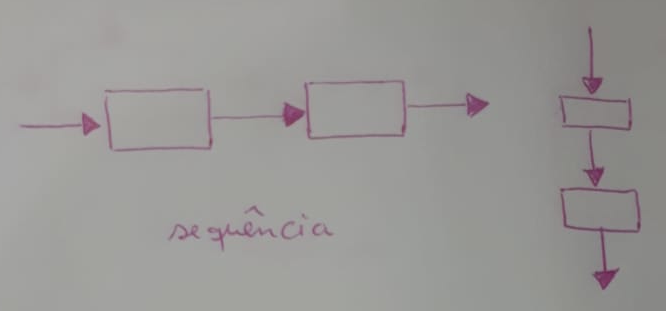
\includegraphics[width=0.7\textwidth]{images/fig-blocos-sequencia.png}
\end{frame}


\begin{frame}{Lógica estruturada}
    \fontsize{12pt}{15}\selectfont{
        Decisão/Condição
	}\par
	\vspace{0.5em}
	\centering
    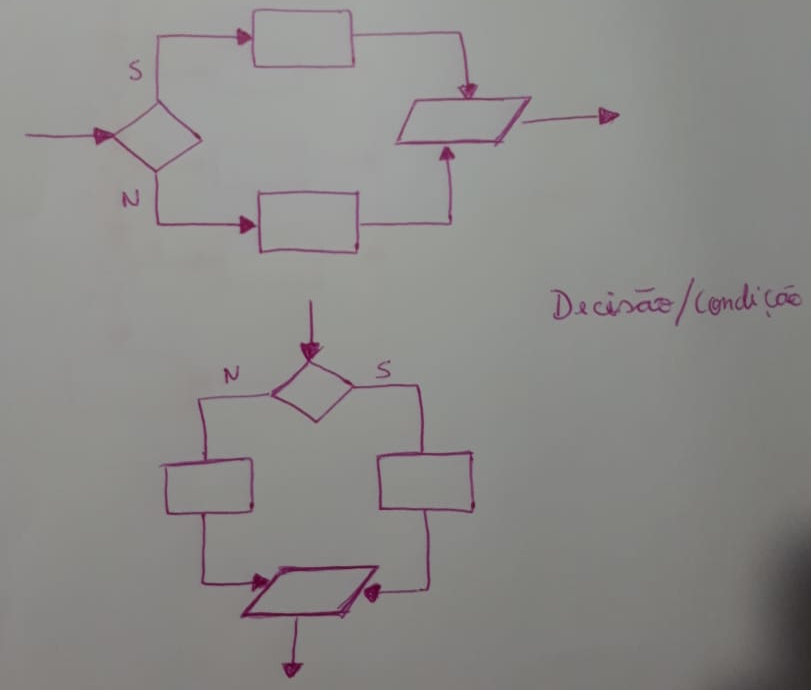
\includegraphics[width=0.6\textwidth]{images/fig-blocos-condicao.png}
\end{frame}


\begin{frame}{Lógica estruturada}
    \fontsize{12pt}{15}\selectfont{
        Repetição
	}\par
	\vspace{1em}
	\centering
    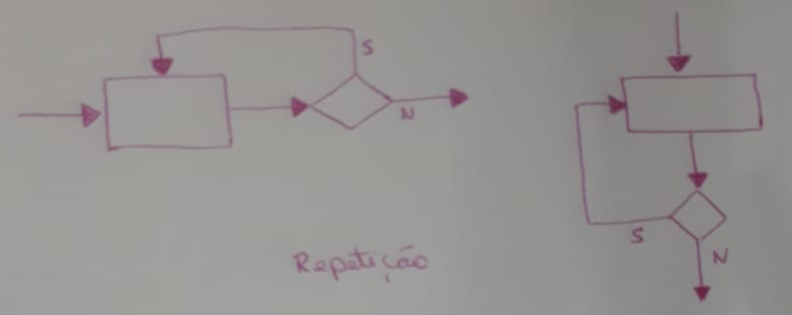
\includegraphics[width=0.7\textwidth]{images/fig-blocos-repeticao.png}
\end{frame}


\begin{frame}{Lógica estruturada}
    \fontsize{12pt}{15}\selectfont{
        Caso
	}\par
	\vspace{1em}
	\centering
    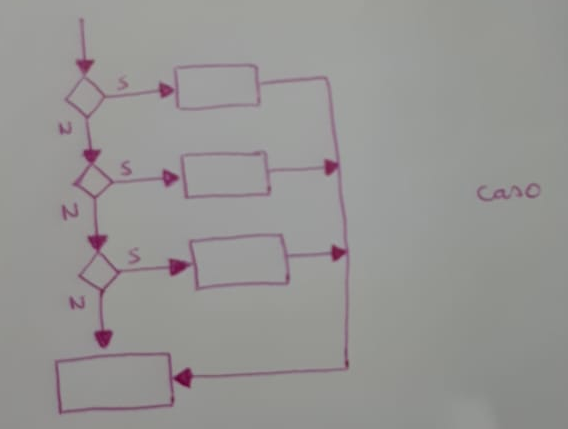
\includegraphics[width=0.6\textwidth]{images/fig-blocos-caso.png}
\end{frame}




\begin{frame}{Lógica Modular}
    \fontsize{12pt}{15}\selectfont{
        A técnica da lógica \textbf{modular} é elaborada como uma estrutura de partes independentes, denominadas de módulos, cujo procedimento segue regras, a saber: 
        
        \vspace{0.5cm}
        
        \begin{itemize}
            \item decompor um diagrama em partes independentes; e
            \item dividir um problema em outros menores.
        \end{itemize}
	}\par
	\vspace{1em}
\end{frame}


\begin{frame}{Lógica modular}
	\vspace{1em}
	\centering
    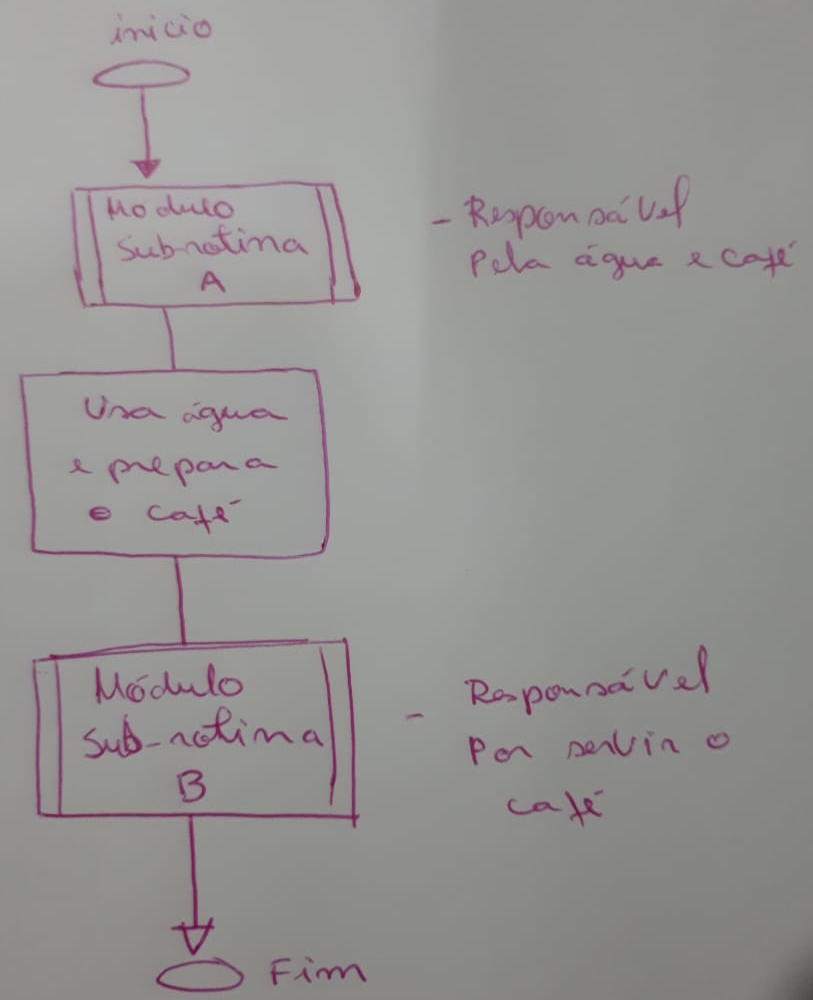
\includegraphics[width=0.45\textwidth]{images/fig-logica-modular.png}
\end{frame}


\begin{frame}{Exercício Lista 2 - Questão 5}
    \fontsize{12pt}{15}\selectfont{
        l2-q5) Utilize diagrama de blocos para resolver o seguir problema: leia três números inteiros e calcule a soma. Considerar que a condição, se a soma for maior que 10, escreva ``tem erro'', do contrário escreva o valor da soma.
	}\par
	\vspace{1em}
\end{frame}

\begin{frame}{Exercício Lista 2 - Questão 5}
	\vspace{1em}
	\centering
    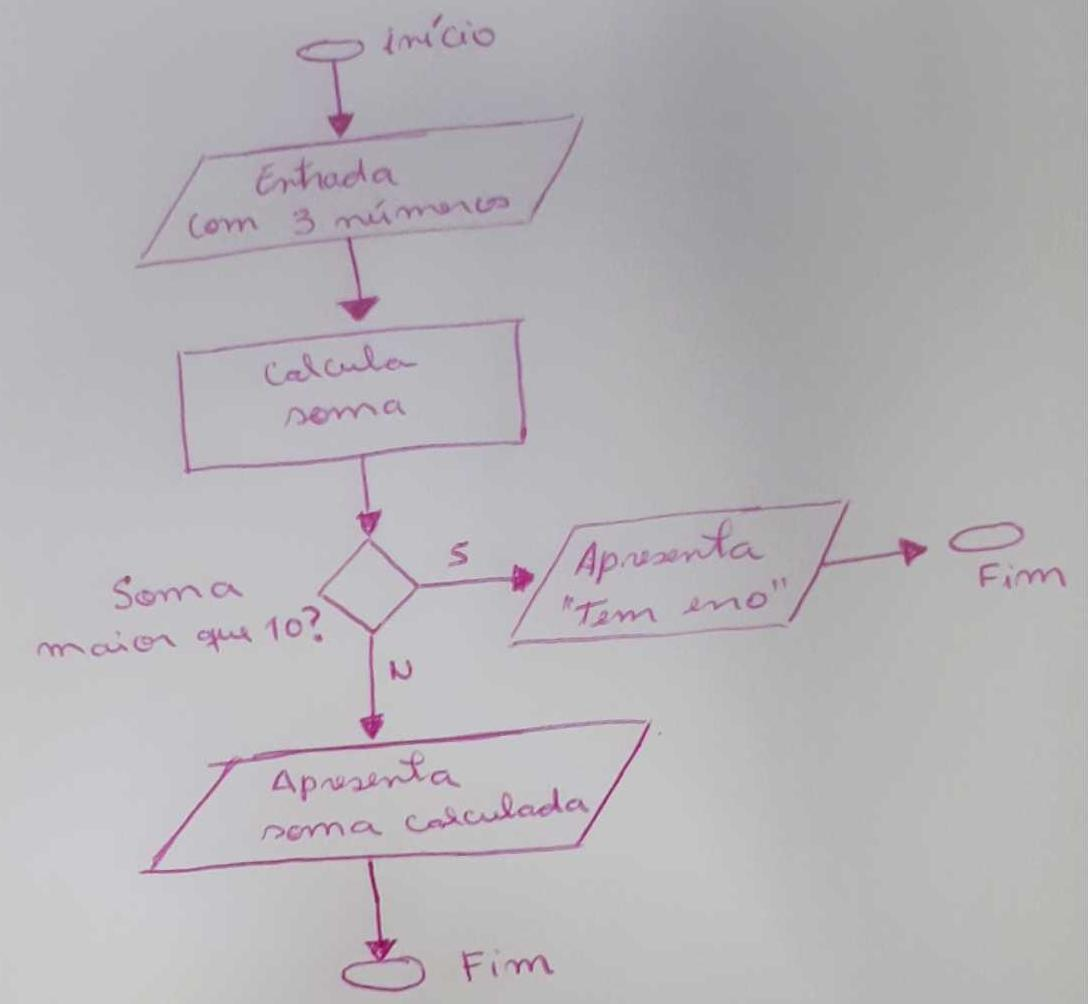
\includegraphics[width=0.55\textwidth]{images/fig-exercicio-02-q5.jpeg}
\end{frame}



\begin{frame}{Exercício Lista 2 - Questão 6}
    \fontsize{12pt}{15}\selectfont{
        l2-q6) Utilize diagrama de blocos para resolver o seguir problema: leia três notas de um aluno, calcule e escreva a média final deste aluno. Considerar que a média é ponderada e que o peso das notas é 2, 3 e 5. 
        \vspace{1cm}
        
        Média Final (MF)~=~$\frac{N1\times 2 + N2 \times 3 + N3 \times 5}{10}$
	}\par
	\vspace{1em}
\end{frame}

\begin{frame}{Exercício Lista 2 - Questão 6}
	\vspace{1em}
	\centering
    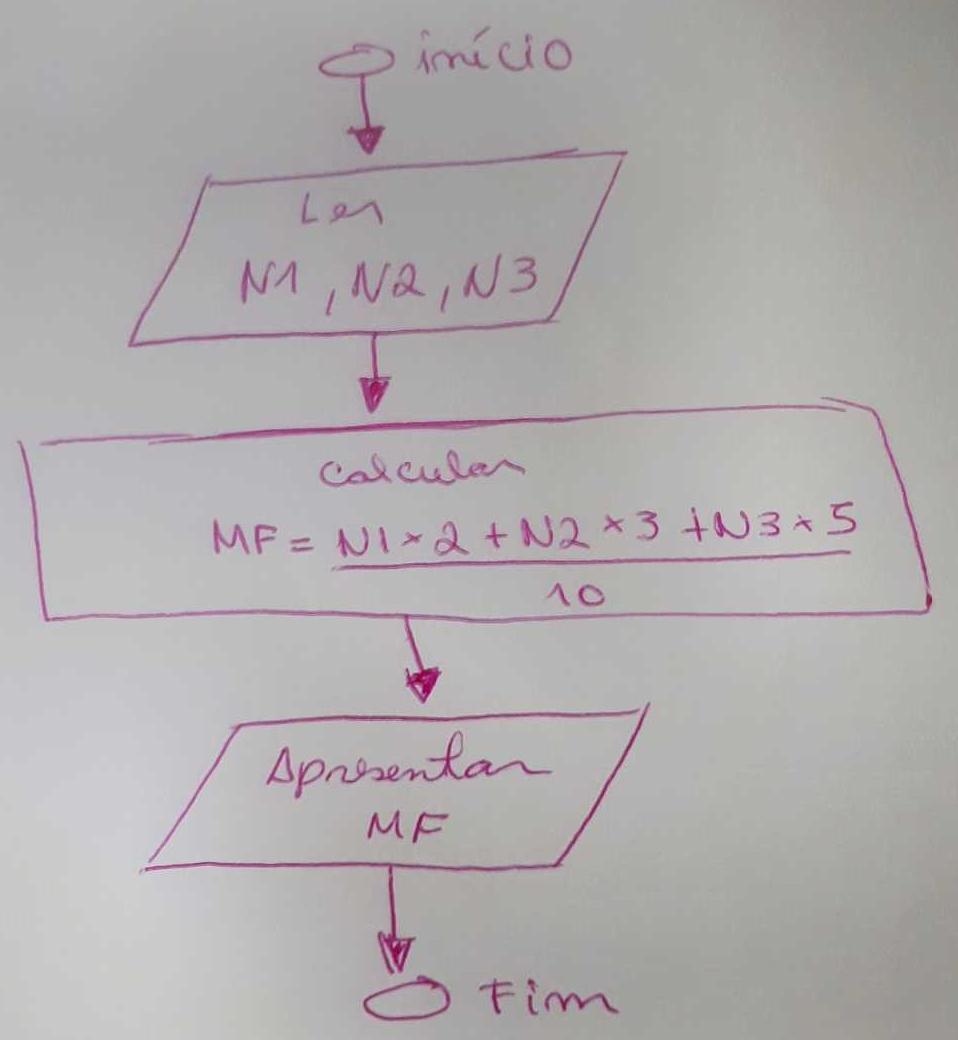
\includegraphics[width=0.5\textwidth]{images/fig-exercicio-02-q6.jpeg}
\end{frame}


\begin{frame}{Exercício Lista 2 - Questão 7}
    \fontsize{12pt}{15}\selectfont{
        l2-q7) Utilize diagrama de blocos para resolver o seguir problema: as maçãs custam R\$ 1,50 cada se forem compradas menos de uma dúzia, e R\$ 1,00 se forem compradas pelo menos 12. leia o número de maçãs compradas, calcule e escreva o custo total da compra. 
        \vspace{1cm}
	}\par
	\vspace{1em}
\end{frame}

\begin{frame}{Exercício Lista 2 - Questão 7}
	\vspace{1em}
	\centering
    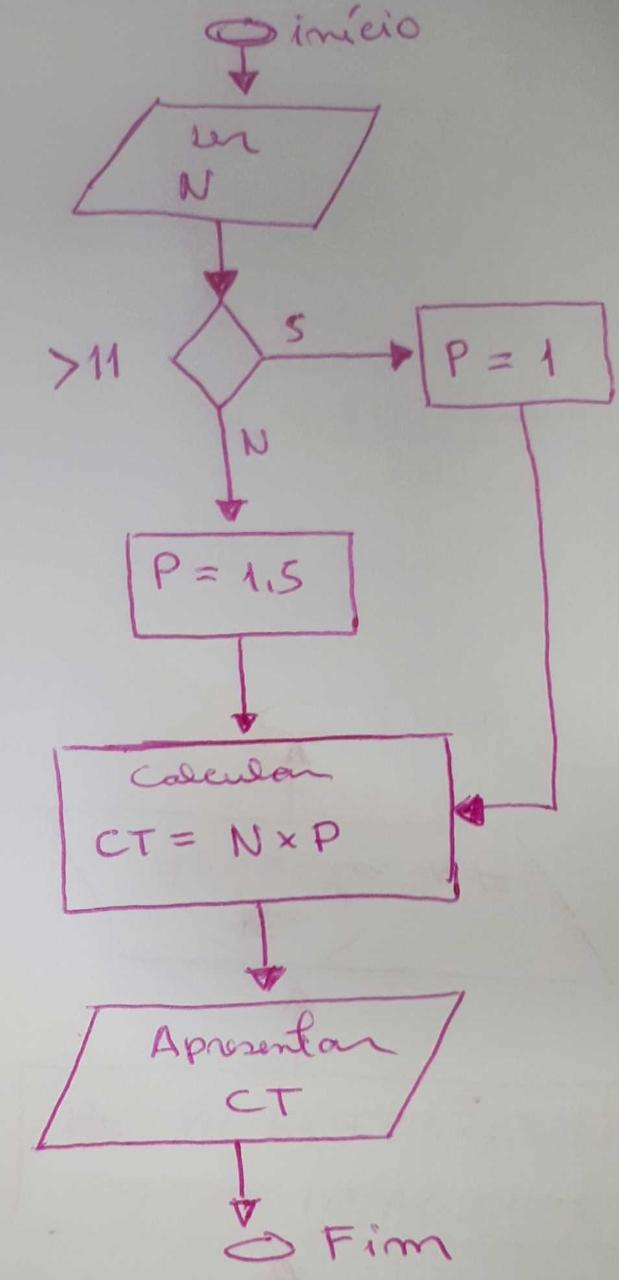
\includegraphics[width=0.3\textwidth]{images/fig-exercicio-02-q7.jpeg}
\end{frame}


\begin{frame}{Exercício Lista 2 - Questão 8}
    \fontsize{12pt}{15}\selectfont{
        l2-q8) Utilize diagrama de blocos para resolver o seguir problema: a jornada de trabalho semanal de um funcionário é de 40 horas. O funcionário que trabalhar mais de 40 horas receberá hora extra, cujo cálculo é o valor da hora regular com um acréscimo de 50\%. leia o número de horas trabalhadas em um mês, o salário por hora e escreva o salário total do funcionário, que deverá ser acrescido das horas extras, caso tenham sido trabalhadas (considere que o mês possua 4 semanas exatas).
        \vspace{1cm}
	}\par
	\vspace{1em}
\end{frame}

\begin{frame}{Exercício Lista 2 - Questão 8}
	\vspace{1em}
	\centering
    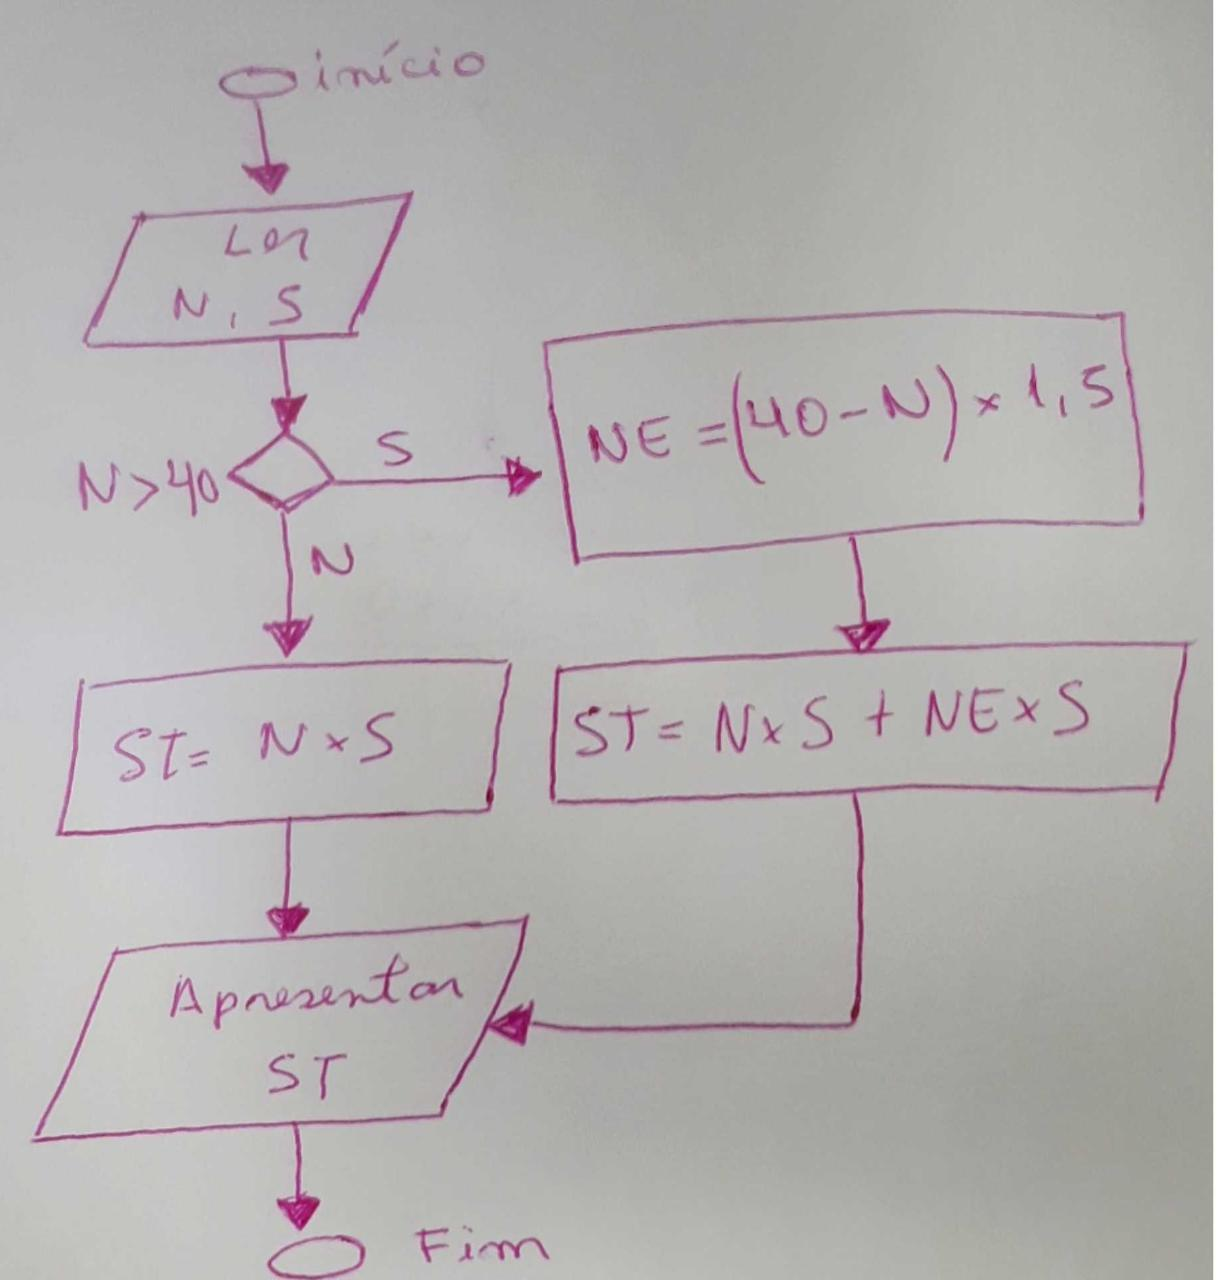
\includegraphics[width=0.5\textwidth]{images/fig-exercicio-02-q8.jpeg}
\end{frame}



\section{Tipos de Dados e Instruções Primitivas}


\begin{frame}{Resumo}
    \fontsize{12pt}{15}\selectfont{
    A partir deste ponto de estudo, teremos contato direto com a parte mais prática desta disciplina. Anteriormente, apresentou-se uma teoria básica de alguns pontos que, por vezes, levaram dúvidas até a alguns profissionais experientes da área de tecnologia da informação.
        
	}\par
	\vspace{1em}
\end{frame}



\begin{frame}{Tipos de informação}
    \fontsize{12pt}{15}\selectfont{
    Daqui pra frente é necessário considerar que um computador é uma ferramenta para solucionar problemas que envolvam a manipulação de informação, as quais se classificam, grosso modo, em dois tipos básicos: dados e instruções.
        
	}\par
	\vspace{1em}
\end{frame}


\begin{frame}{Tipos de dados}
    \fontsize{13pt}{15}\selectfont{
    Os dados são representados por elementos advindos do mundo externo, os quais representam as informações que os seres humanos manipulam. Eles devem ser abstraídos para serem processados em um computador. Os dados podem ser categorizados em três tipos: numéricos, caracteres e lógicos.
        
	}\par
	\vspace{1em}
\end{frame}


\begin{frame}{Tipos de dados}
    \fontsize{13pt}{15}\selectfont{
        \begin{itemize}
            \item \textbf{Numéricos} - representados por valores inteiros ou reais.
            \item \textbf{Caracteres} - representados por valores alfabéticos ou alfanuméricos os quais não são utilizados em operações de cálculo matemático.
            \item \textbf{Lógicos} - representados por valores dos tipos falsos ou verdadeiro.
        \end{itemize}
        
	}\par
	\vspace{1em}
	*Os tipos de dados \textbf{numérico inteiro}, \textbf{numérico real}, \textbf{caracteres} e \textbf{lógico} são conhecidos como tipos de \textbf{dados primitivos} ou tipos de \textbf{dados básicos}.
	\vspace{1em}
\end{frame}

\begin{frame}{Tipos de dados NUMÉRICOS}
    \fontsize{13pt}{15}\selectfont{
        São tipos de dados numéricos possuem duas classes, números inteiros e reais.
	}\par
	\fontsize{12pt}{15}\selectfont{
	    \begin{itemize}
	        \item \textbf{INTEIRO} - são inteiros os dados numéricos positivos e negativos pertencentes ao \textbf{conjunto de números inteiros}, excluindo qualquer valor numérico fracionário, como por exemplo: R\$ 3,19 (não inteiro, fracionário).
	        
	        \item \textbf{REAL} - são reais os dados numéricos positivos e negativos pertencentes ao \textbf{conjunto de números reais}, incluindo todos os valores fracionários e também os valores inteiros, como por exemplo: R\$ 3,19 (não inteiro, fracionário, real).
	    \end{itemize}
	}\par
	\vspace{1em}
\end{frame}


\begin{frame}{Tipo de dados - CARACTERES}
    \fontsize{12pt}{15}\selectfont{
        Os tipos de caracteres são sequência de valores delimitados por aspas formadas por letras de (A até Z), números (|de 0 até 9|) e símbolos - todos os símbolos do teclado. Ele também é conhecido como \textbf{alfanumérico}, \textbf{string} (em inglês - cordão, colar), \textbf{literal} ou \textbf{cadeia}.
        
        Por exemplo, ``Rua João e Maria''.
        
	}\par
	\vspace{1em}
\end{frame}


\begin{frame}{Tipo de dados - LÓGICOS}
    \fontsize{12pt}{15}\selectfont{
        São lógicos os dados com valores que sugerem uma única opção entre duas possibilidades existentes, normalmente representados pelos valores \textbf{FALSO} ou \textbf{VERDADEIRO}, podendo também ser representados por \textbf{SIM} ou \textbf{NÃO}, \textbf{1 (um)} ou \textbf{0 (zero)}, entre outros, desde que mantida a relação de escolher apenas uma das duas opções de possibilidade existentes. 
        
        Ele também é conhecido por \textbf{booleano}, devido à contribuição de George Boole.
	}\par
	\vspace{1em}
\end{frame}


\begin{frame}{O uso de variáveis}
    \fontsize{12pt}{15}\selectfont{
        Tem-se como definição de variável tudo aquilo que é sujeito a variação, que é incerto, instável ou inconstante.
        
        \vspace{1em}
        Para utilizar o conceito de variável, imagine que a memória de um computador é um grande arquivo com várias gavetas, e cada gaveta pode armazenar um único valor (seja ele numérico, caractere ou lógico).
	}\par
	\vspace{1em}
\end{frame}


\begin{frame}{O uso de variáveis}
	\vspace{1em}
	\centering
    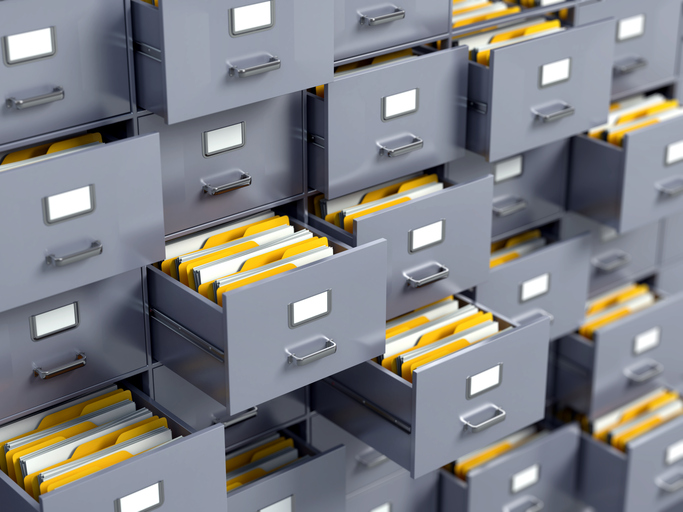
\includegraphics[width=0.7\textwidth]{images/fig-gavetas.jpg}
\end{frame}


\begin{frame}{O uso de variáveis}
    \fontsize{14pt}{15}\selectfont{
        Se a memória do computador for comparado a um grande arquivo com várias gavetas, e em cada gaveta é possível guardar um único valor por vez. Como em um arquivo, as gavetas devem estar identificadas com uma etiqueta contendo um nome. 
        \vspace{1em}
        
        Você há de concordar que é necessário identificar com um nome a gaveta que se pretende utilizar. Desta forma o valor armazenado pode ser utilizado a qualquer momento.
        
	}\par
	\vspace{1em}
\end{frame}


\begin{frame}{O uso de variáveis}
	\vspace{1em}
	\centering
    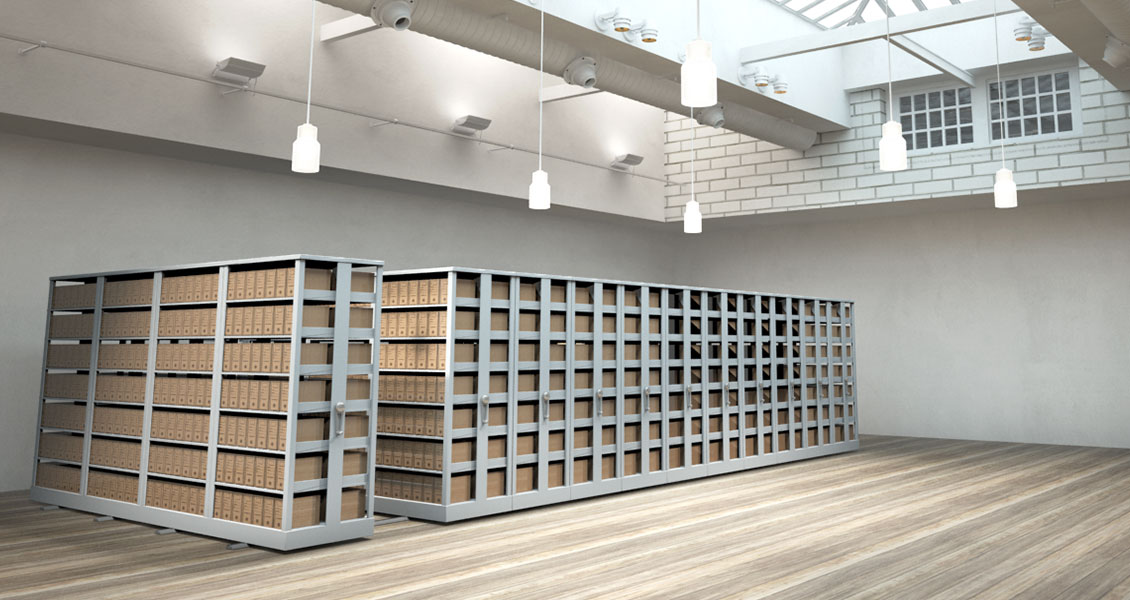
\includegraphics[width=0.8\textwidth]{images/fig-arquivo-gavetas.jpg}
\end{frame}




\begin{frame}{O uso de variáveis}
    \fontsize{14pt}{15}\selectfont{
        O nome de uma variável é utilizado para sua identificação e representação dentro de um programa de computador. É necessário estabelecer e seguir algumas regras de definição e uso de variáveis, a saber:
        
        \vspace{1em}
	}\par
	\fontsize{12pt}{15}\selectfont{
	    \begin{itemize}
	        \item Os nomes de identificação de uma variável podem utilizar um ou mais caracteres, limitando-se a restrição da própria linguagem formal de programação em uso. No caso do diagrama de blocos essa restrição não existe.
	    \end{itemize}
	}
	\vspace{1em}
\end{frame}


\begin{frame}{O uso de variáveis}
    \fontsize{14pt}{15}\selectfont{
        (continuação)
        \vspace{1em}
	}\par
	\fontsize{12pt}{15}\selectfont{
	    \begin{itemize}
	        \item O primeiro caractere de identificação do nome de uma variável não pode ser, em hipótese alguma, numérico. O primeiro caractere de identificação do nome de uma variável deve sempre ser alfabético, os demais podem ser alfanuméricos.
	        
	        \item Na definição de um nome composto de uma variável não podem existir espaços em branco entre os nomes. 
	        
	        \item Jamais uma variável pode ser definida com o mesmo nome de uma palavra que representa os comandos de uma linguagem de programação de computador, ou seja, com as palavras reservadas de uma linguagem.
	        
	    \end{itemize}
	}
	\vspace{1em}
\end{frame}



\begin{frame}{O uso de variáveis}
    \fontsize{14pt}{15}\selectfont{
        Por fim, do ponto de vista computacional pode-se definir uma variável de forma bem simplista como uma representação de uma região de memória utilizada para armazenar um determinado valor por um espaço de tempo. O tempo de armazenamento de um valor está relacionado ao tempo de duração da execução de um programa.
        \vspace{1em}
	}\par
	\vspace{1em}
\end{frame}


\begin{frame}{O uso de constantes}
    \fontsize{14pt}{15}\selectfont{
        \textbf{Constante} é tudo que é fixo, estável, inalterável, imutável, contínuo, invariável, de um valor fixo e que é aplicado sob diversos pontos de vista. Assim sendo, do ponto de vista computacional, que é semelhante ao matemático ou científico, uma constante é uma grandeza numérica que mantém-se inalterado.
        \vspace{1em}
	}\par
	\vspace{1em}
\end{frame}



\begin{frame}{Os operadores aritméticos}
    \fontsize{12pt}{15}\selectfont{
        Os operadores aritméticos são as ferramentas responsáveis pelo estabelecimento das operações matemáticas a serem realizadas em um computador. Tanto variáveis como constantes são utilizadas na elaboração dos cálculos matemáticos. Eles são classificados em:
        \vspace{1em}
	}\par
	\fontsize{12pt}{15}\selectfont{
	    \begin{itemize}
	        \item \textbf{unários} - quando atuam na inversão do estado de um valor numérico, que pode este ser passado de positivo para negativo ou de negativo para positivo; ou
	        
	        \item \textbf{binários} - quando utilizados em operações matemáticas de exponenciação, divisão, multiplicação, adição e substração.
	        
	    \end{itemize}
	}
	\vspace{1em}
\end{frame}




\begin{frame}{Os operadores aritméticos}

\resizebox{\linewidth}{!}{
\begin{tabular}{|c|c|c|c|c|}
\hline
\textbf{Operador} & \textbf{Operação}& \textbf{Categoria} & \textbf{Prioridade} & \textbf{Resultado} \\ \hline
=  & Atribuição & -o- & -o-  & -o- \\ \hline
+  & Manutenção de sinal & unário & 1 & -o- \\ \hline
-  & Inversão de sinal& unário & 1 & -o- \\ \hline
\textasciicircum{}& Exponenciação & binário& 2 & inteiro ou real \\ \hline
% \textasciicircum{}(1/n) & Radiciação de índice n & binário& 2 & real\\ \hline
/  & Divisão & binário& 3 & real \\ \hline
*  & Multiplicação & binário& 3 & inteiro ou real \\ \hline
+  & Adição  & binário& 4 & inteiro ou real \\ \hline
-  & Subtração  & binário& 4 & inteiro ou real \\ \hline
\end{tabular}
}

*o quadro apresenta os operadores aritméticos segundo a ordem de prioridade matemática em que as operações aritméticas são realizadas. Para alterar o nível de prioridade deve utilizar-se parênteses. Por exemplo, X = 10 * 10 + 2 e Y = 10 * (10 + 2), X tem resultado 102 e Y tem resultado 120.

\end{frame}


\begin{frame}{Instruções Básicas}
    \fontsize{12pt}{15}\selectfont{
        As instruções a serem implementadas para execução de um determinado programa são representadas por um conjunto de palavras-chave (vocabulário). Uma instrução pode se:
        \vspace{1em}
	}\par
	\fontsize{12pt}{15}\selectfont{
	    \begin{itemize}
	        \item \textbf{formal} - quando baseia-se em linguagem real de programação de computadores, tais como C, Java, PHP; ou
	        
	        \item \textbf{informal} - quando baseia-se em pseudocódigo, como é o caso da linguagem usada até, diagrama de blocos.
	        
	    \end{itemize}
	}
	\vspace{1em}
\end{frame}



\begin{frame}{Entrada, Processamento e saída}
    \fontsize{12pt}{15}\selectfont{
        Para criar um programa que seja executável dentro de um computador, é preciso ter em mente três pontos de trabalho:
        \vspace{1em}
	}\par
	\fontsize{12pt}{15}\selectfont{
	    \begin{itemize}
	        \item entrada de dados - alimenta o programa;
	        
	        \item processamento - processa a(s) entrada(s); e
	        
	        \item saída de dados - apresenta o resultado.
	        
	    \end{itemize}
	}
	\vspace{1em}
\end{frame}


\section{Introdução à linguagem c}

\begin{frame}{Meu primeiro programa}
    \fontsize{12pt}{15.2}\selectfont{
	Estrutura básica de um programa em C. 
	
	Code::Blocks IDE \url{www.codeblocks.org}
		
	\vspace{0.5em}
	\centering
    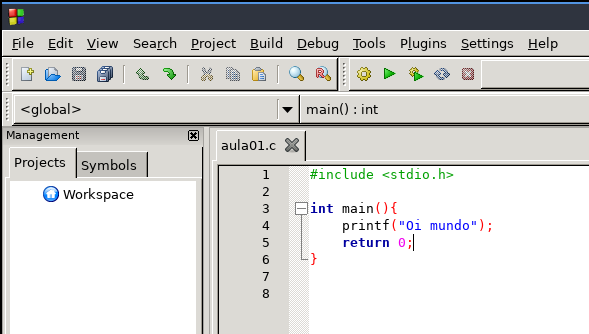
\includegraphics[width=0.75\textwidth]{images/fig-aula01-oi-mundo.png}

    }\par

	\vspace{1em}
\end{frame}

\begin{frame}[fragile]{Programa 001}

\lstinputlisting[style=CBruno,caption=Exemplo de Código]{codigos/c/001-oimundo.c}

\end{frame}

\begin{frame}{Meu primeiro programa}
    \fontsize{12pt}{15.2}\selectfont{
	Estrutura básica de um programa em C.
		
	\vspace{1em}
	\centering
    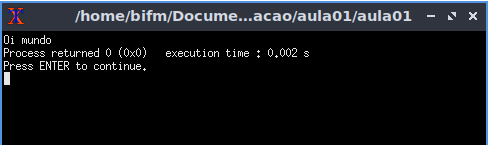
\includegraphics[width=0.8\textwidth]{images/fig-aula01-oi-mundo-p2.png}

    }\par

	\vspace{1em}
\end{frame}


\begin{frame}{Comentário}
    \fontsize{12pt}{15.2}\selectfont{
	São blocos de códigos ignorados pelo compilador.
		
	\vspace{1em}
	// comentário de linha
	
	/*
	
	comentário de bloco
	
	*/
	
    }\par

	\vspace{1em}
\end{frame}



\begin{frame}{Identação}
    \fontsize{14pt}{15.2}\selectfont{
	Identar um código nada mais é que separar os códigos em blocos através de tabulação.
		
	\vspace{1em}
	Não identado:
	
	\#include <stdio.h>int main()\{printf(``Oi mundo'');return 0;\}
	

    }\par
    
    \vspace{1em}
    
    *O código acima não está identado. Note como está complicado de ler, apesar de ser um código extremamente simples.
    
	\vspace{1em}
\end{frame}

\begin{frame}{Tipos de Dados}
    \fontsize{14pt}{15.2}\selectfont{
    
	A linguagem C possuí 5 (cinco) tipos básicos de dados: \textbf{char}, \textbf{int}, \textbf{float}, \textbf{void} e \textbf{double}.
	
	\vspace{1em}
	
	O \textbf{void} é um tipo de dado vazio (sem valor).
	
	\vspace{1em}
	
	Para cada tipo de dado existem modificadores de tipo, estes são 4 (quatro): \textbf{signed}, \textbf{unsigned}, \textbf{long} e \textbf{short}.
	
	\vspace{1em}
	
	Para o \textbf{float} nenhum modificado pode ser aplicado; assim como para o \textbf{double} podemos aplicar APENAS o \textbf{long}.
		
    }\par
    
    \vspace{1em}

\end{frame}


\begin{frame}{Tipos de Dados}
    \fontsize{14pt}{15.2}\selectfont{
    
	\begin{tabular}{|l|l|l|}
	\hline
Nome & Característica  & Intervalo \\ \hline
\textbf{char} & carácter/literal  &  -128 a 127  \\ \hline
\textbf{int} & número inteiro & -32.768 a 32.767  \\ \hline
\textbf{float} & ponto flutuante em simples precisão  & 3.4 E-38 a 3.4E+38 \\ \hline
\textbf{double} & ponto flutuante em dupla precisão  & 1.7 E-308 a 1.7E+308  \\ \hline
\textbf{void} & vazio & (sem valor)   \\ \hline

\end{tabular}
		
    }\par
    
    \vspace{1em}

\end{frame}


\begin{frame}{Tipos de Dados}
    \fontsize{14pt}{15.2}\selectfont{
    Qualificadores de tipo \textbf{unsigned} e \textbf{signed} podem ser aplicados a tipos \textbf{char} e \textbf{int}:
    
    \vspace{5mm}
    
    \textbf{unsigned} - considera apenas valores positivos.
    
    \vspace{5mm}
    
    
    \textbf{signed} - consideram valores positivos e negativos. por padrão todos são signed.
		
    }\par
    
    \vspace{1em}

\end{frame}

\begin{frame}{Tipos de Dados}
    \fontsize{14pt}{15.2}\selectfont{
    Qualificadores de tipo \textbf{long} e \textbf{shot} podem ser aplicados a tipos \textbf{int} e \textbf{double}. Entretanto, para \textbf{double}, apenas o \textbf{long} é aplicado.
    
    \vspace{5mm}
    
    \textbf{short} - aplicável apenas para \textbf{int}. Reduz pela metade o tamanho.
    
    \vspace{5mm}
    
    
    \textbf{long} - aplicável para \textbf{int} e \textbf{double}.
		
    }\par
    
    \vspace{1em}

\end{frame}



\begin{frame}{Tipos de dados}
	\vspace{1em}


\begin{tabular}{|l|r|c|r|r|}
\hline
\multirow{2}{*}{Tipo} & Número & 
Formato  & \multicolumn{2}{c|}{Intervalo}\\ 

& de bytes & Sintaxe printf & 
Início & Fim \\ \hline 

char& 1& \%c & -128 & 127 \\ \hline
unsigned char & 1& \%c & 0& 255 \\ \hline
signed char & 1& \%c & -128 & 127 \\ \hline
int & 4 & \%d & -32.768& 32.767\\ \hline
unsigned int& 4 & \%u & 0& 65.535\\ \hline
signed int& 2 & \%i & -32.768& 32.767\\ \hline
short int & 2 & \%hi& -32.768& 32.767\\ \hline
unsigned short int& 2 & \%hu& 0& 65.535\\ \hline
signed short int& 2 & \%hi& -32.768& 32.767\\ \hline
long int& 8 & \%li& -2.147.483.648 & 2.147.483.647 \\ \hline
signed long int & 8 & \%li& -2.147.483.648 & 2.147.483.647 \\ \hline
unsigned long int & 8 & \%lu& 0& 4.294.967.295 \\ \hline
double & 8 & \%d& - & - \\ \hline
long double & 16 & \%d& - & - \\ \hline
float & 4 & \%f & - & - \\ \hline
long (inteiro) & 4 & \%f & - & - \\ \hline
short (inteiro) & 2 & \%f & - & - \\ \hline
\end{tabular}

	
% 	\centering
%     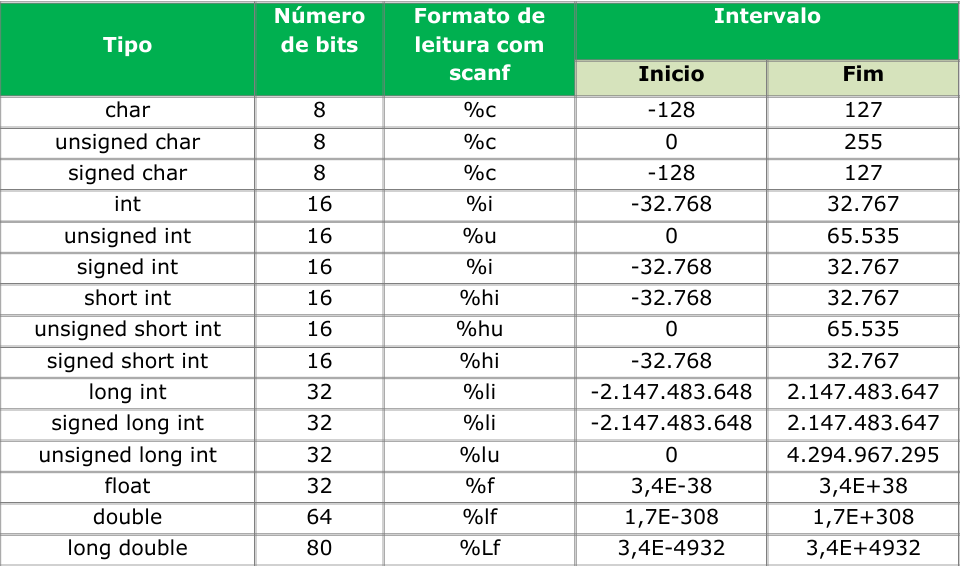
\includegraphics[width=0.85\textwidth]{images/fig-tipo-de-dados.png}
\end{frame}


\begin{frame}{Tipos de Dados}
    \fontsize{14pt}{15.2}\selectfont{
    \textbf{Declaração de variável}: 
    \vspace{1em}
    }\par
    \fontsize{12pt}{15.2}\selectfont{
        tipo\_da\_variavel nome\_da\_variavel = valor\_inicial\_da\_variavel; 
	}
    
    \vspace{1em}

    \fontsize{14pt}{15.2}\selectfont{
    \textbf{Declaração de variáveis de um mesmo tipo}: 
    \vspace{1em}
    }\par
    \fontsize{12pt}{15.2}\selectfont{
        tipo\_da\_variavel nome\_da\_variavel1 = valor1, nome\_var2 = valor2; 
	}

	\vspace{1em}
\end{frame}

\begin{frame}{Boas práticas}
    \fontsize{16pt}{15.2}\selectfont{
    Ao nomear uma variável seja objetivo, use nomes fáceis de entender e se necessário faça um comentário acima da variável explicando sua utilidade. Em nomes compostos separe-os utilizando underline.
    \vspace{1em}
    }
\vspace{1em}

\end{frame}


\begin{frame}{Constantes de barra invertida}

\begin{tabular}{|c|l|}
\hline
\textbf{Constante}                        & \textbf{Representação}   \\ \hline
\textbackslash{}n                & Nova Linha      \\ \hline
\textbackslash{}t                & Tab Horizontal  \\ \hline
\textbackslash{}v                & Tab Vertical    \\ \hline
\textbackslash{}"                & Aspas Duplas    \\ \hline
\textbackslash{}'                & Aspas Simples   \\ \hline
\textbackslash{}\textbackslash{} & Barra Invertida \\ \hline
\textbackslash{}a                & Sinal sonoro/Beep     \\ \hline

\end{tabular}


	\vspace{1em}
\end{frame}


\begin{frame}{Operadores aritméticos e de atribuição}

\begin{tabular}{|c|l|}
\hline
\textbf{Operador} & \textbf{Ação}   \\ \hline
+ & Soma      \\ \hline
- & Substração  \\ \hline
* & Multiplicação    \\ \hline
/ & Divisão     \\ \hline
\%  & Resto da divisão   \\ \hline
++ & Incremento\\ \hline
-- & Decremento     \\ \hline

\end{tabular}


	\vspace{1em}
\end{frame}



\begin{frame}{Operadores de Racionais/lógicos}


\begin{tabular}{|c|l|}
\hline
\textbf{Operador} & \textbf{Ação}   \\ \hline
> & Maior do que      \\ \hline
>= & Maior ou igual a  \\ \hline
< & Menor do que    \\ \hline
<= & Menor ou igual a     \\ \hline
==  & Igual a   \\ \hline
!= & Diferente de\\ \hline
\&\& & AND (E) \\ \hline
|| & OR (OU) \\ \hline
! & NOT (NÃO) \\ \hline

\end{tabular}

	\vspace{1em}
\end{frame}

\begin{frame}{Tabela verdade}
    \fontsize{12pt}{15.2}\selectfont{
	\vspace{1em}
	\centering
    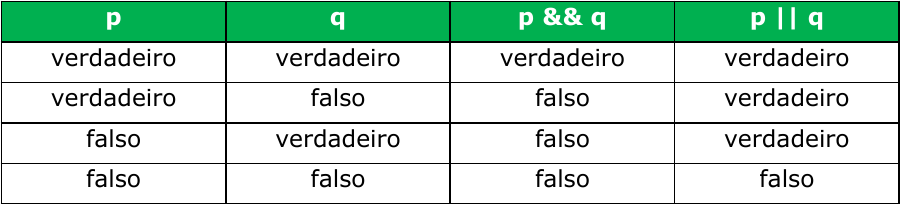
\includegraphics[width=0.8\textwidth]{images/fig-tabela-verdade.png}

    }\par

	\vspace{1em}
\end{frame}


\begin{frame}{Tabela de Precedência}
    \fontsize{12pt}{15.2}\selectfont{
	\vspace{1em}
	\centering
    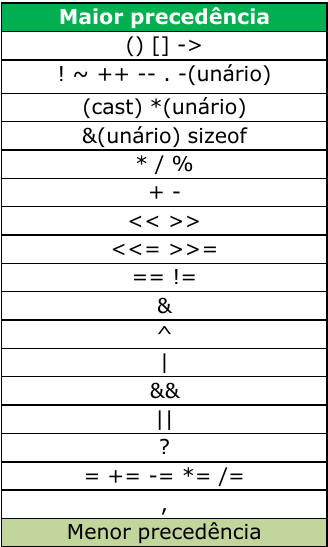
\includegraphics[width=0.35\textwidth]{images/fig-tabela-precedencia.png}

    }\par

	\vspace{1em}
\end{frame}



\begin{frame}{Resolução L3Q7}
    \fontsize{12pt}{15.2}\selectfont{
	Resolução da questão 7 (Q7), lista 3 (L3).
		
	\vspace{0.5em}
	\centering
    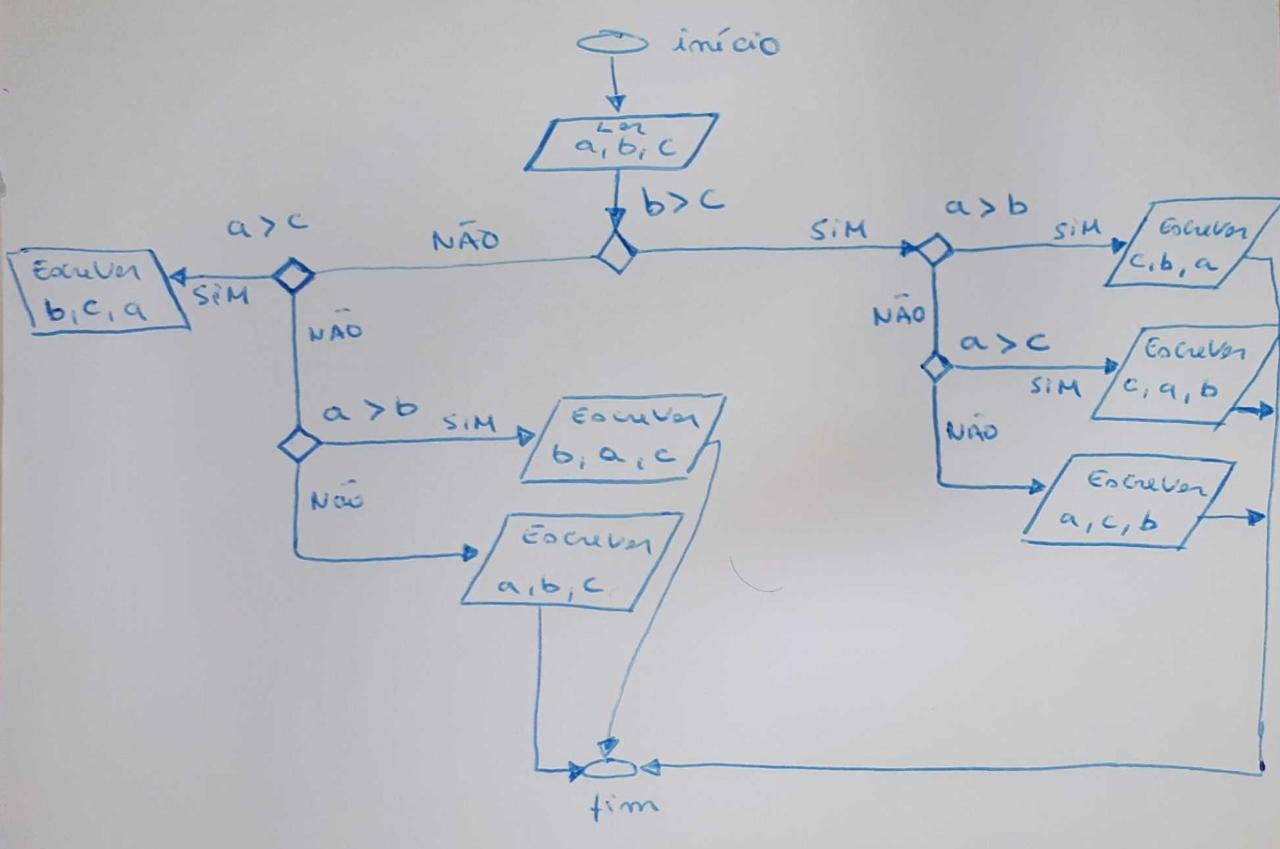
\includegraphics[width=0.7\textwidth]{images/fig-l3-q7.jpeg}

    }\par

	\vspace{1em}
\end{frame}


\begin{frame}{Entrada e saída de dados}
    \fontsize{14pt}{15.2}\selectfont{
    
    \vspace{5mm}
    
    \textbf{scanf(), gets(), fgets()} - utilizados para entrada de dados.
    
    \vspace{5mm}
    
    
    \textbf{printf()} - utilizado para saída de dados.
		
    }\par
    
    \vspace{1em}

\end{frame}



\begin{frame}{Entrada e saída de dados}

\begin{tabular}{|c|l|}
\hline
\textbf{Código} & \textbf{Formado}   \\ \hline
\%c & Receber um caractere      \\ \hline
\%d & Receber número inteiro  \\ \hline
\%f & Receber número de ponto flutuante   \\ \hline
\%s & Receber uma cadeira de caracteres    \\ \hline

\end{tabular}


\end{frame}


\begin{frame}{Entrada e saída de dados}
    \fontsize{13pt}{14}\selectfont{
    
    \vspace{5mm}
    
    \textbf{scanf()} - a entrada é finalizada assim que um espaço em branco (whitespace) é encontrado. É possível burlar usando scanf(``\%[$\text{\^{}}$$\textbackslash$n]s'', x) % , newline ou EOF.
    
    \vspace{5mm}
    
    \textbf{gets()} - considera um espaço em branco como parte da cadeia de entrada e termina a entrada ao encontrar newline ou EOF.
    
    \vspace{5mm}
    
    % \textbf{fgets()} - mais confiável que os outros dois, ele evita erros de estouro de buffer, minimizando riscos de segurança. Porém, insere uma quebra de linha ao final.
		
    }\par
    
    \vspace{1em}

\end{frame}


\begin{frame}[fragile]{Exemplo 002}

\lstinputlisting[style=CBruno,caption=Exemplo de Código]{codigos/c/002-scanf.c}

\end{frame}

\begin{frame}[fragile]{Exemplo 003}

\lstinputlisting[style=CBruno,caption=Exemplo de Código]{codigos/c/003-gets.c}

\end{frame}

% \begin{frame}[fragile]{Entrada e saída de dados}

% \lstinputlisting[style=CBruno,caption=Exemplo de Código]{codigos/c/004-fgets.c}

% \end{frame}



\begin{frame}{Estruturas de Controle de Fluxo}
    \fontsize{14pt}{14}\selectfont{
    
        \begin{itemize}
            \item São responsáveis por controlar o fluxo do programa 
            \item Testam condições. 
            \item Algumas são conhecidas como ``loops''.
        \end{itemize}
    }\par
    \vspace{1em}
\end{frame}




\begin{frame}{if-else}
    \fontsize{14pt}{14}\selectfont{
    A estrutura \textbf{if-else} é utilizada para tomada de decisões, quando uma condição é válida ou não.
         \vspace{1em}
        
        if ( condicao ) \{ 
        
        \hspace{5mm}    bloco\_de\_comando 
            
        \} else \{ 
        
        \hspace{5mm}    bloco\_de\_comando 
            
        \}
        
    }\par
    \vspace{1em}
\end{frame}

\begin{frame}[fragile]{Exemplo 004}

\lstinputlisting[style=CBruno,caption=Exemplo de Código]{codigos/c/004-if-else.c}

\end{frame}




\begin{frame}{switch}
    \fontsize{13pt}{14}\selectfont{
    O \textbf{switch} também é utilizado para tomada de decisões, porém cria um código mais limpo. Com ele você pode testar uma variável em relação a diversos valores pré- estabelecidos.
    
         \vspace{1em}
        
        switch ( variável ) \{ 
        
        \hspace{5mm}   case 1:
        
        \hspace{5mm}\hspace{5mm}    bloco\_de\_comando 
        
        \hspace{5mm} \hspace{5mm} break;
        
        \hspace{5mm} default: 
        
        \hspace{5mm}\hspace{5mm}    bloco\_de\_comando 
            
        \}
        
    }\par

\end{frame}


\begin{frame}[fragile]{Exemplo 005}

\lstinputlisting[style=CBruno,caption=Exemplo de Código]{codigos/c/005-switch.c}

\end{frame}


\begin{frame}{switch}
    \fontsize{14pt}{14}\selectfont{
    *obs: trabalha com números inteiros.
        
    }\par
    \vspace{1em}
\end{frame}

\begin{frame}{while}
    \fontsize{14pt}{14}\selectfont{
    O \textbf{while} é uma estrutura de repetição, utilizada para criar os chamados ``loops'' de um programa. O código dentro do bloco repetirá enquanto a condição não for verdadeira.
    
         \vspace{1em}
        
        while ( condicao ) \{ 

        \hspace{5mm}   bloco\_de\_comando 
            
        \}
        
    }\par
      \vspace{1em}
      
    *É utilizando quando não sabe-se a quantidade de repetições.
  
\end{frame}

\begin{frame}[fragile]{Exemplo 006}

\lstinputlisting[style=CBruno,caption=Exemplo de Código]{codigos/c/006-while.c}

\end{frame}



\begin{frame}[fragile]{for}
    \fontsize{14pt}{14}\selectfont{
   Assim como o \textbf{while} o \textbf{for} é utilizado para criar estruturas de repetição.
    
         \vspace{1em}
        
        for ( inicializacao; condicao; incremento ) \{ 

        \hspace{5mm}   bloco\_de\_comando 
            
        \}
        
    }\par
    
    %Document body
\begin{lstlisting}[style=CBruno]
for(i=0; i < 10; i++){
    //bloco de comando
}
\end{lstlisting}

    \vspace{1em}
\end{frame}

\begin{frame}[fragile]{Exemplo 007}

\lstinputlisting[style=CBruno,caption=Exemplo de Código]{codigos/c/007-for.c}

\end{frame}


\section{Ambiente de desenvolvimento}

\begin{frame}{}
    \fontsize{12pt}{15}\selectfont{
    \begin{itemize}
        \item Funcionamento; e 
        \item configuração do ambiente para execução;
    \end{itemize}
	}\par
	\vspace{1em}
\end{frame}


% \input{secoes/arquitetura-aplicacoes-multimidia.tex}
% \input{secoes/dispositivos-entrada-saida-multimidia.tex}
% \input{secoes/fundamentos-processamento-imagem.tex}
% \input{secoes/fundamentos-animacao.tex}
% \input{secoes/fundamentos-processamento-som.tex}

% \part{Conteúdo~da~prova~II}
% \frame{\partpage}

% \section{Critérios de seleção de soluções multimídia}
% \section{Recursos básicos de software de autoria}
% \section{Noções de ambientes de realidade virtual}


% \input{secoes/dml-select.tex}

% \section{Objetivos}
% \section{Instruções SQL}
% \section{Considerações Finais}
% Paradigma Relacional
% SGBD e SGBDR
% SQL ANSI e SQL-2003
% \section{Instruções SQL}
% % [DML, DDL, DCL, DTL, DQL]
% \section{SGBD que usam SQL}
% % [MySQL, PostgreSQL, SQLite, Oracle, etc]
% \section{Recuperando dados com instrução Select}
% -Cláusulas
% -Operadores Lógicos
% -Operadores Relacionais
% -Funções de Agregação
% \section{}
% \section{}
% \section{}
% \section{}
% \section{}

% Instruções SQL (DML, DDL, DCL, DTL, DQL)




